\documentclass[1p]{elsarticle_modified}
%\bibliographystyle{elsarticle-num}

%\usepackage[colorlinks]{hyperref}
%\usepackage{abbrmath_seonhwa} %\Abb, \Ascr, \Acal ,\Abf, \Afrak
\usepackage{amsfonts}
\usepackage{amssymb}
\usepackage{amsmath}
\usepackage{amsthm}
\usepackage{scalefnt}
\usepackage{amsbsy}
\usepackage{kotex}
\usepackage{caption}
\usepackage{subfig}
\usepackage{color}
\usepackage{graphicx}
\usepackage{xcolor} %% white, black, red, green, blue, cyan, magenta, yellow
\usepackage{float}
\usepackage{setspace}
\usepackage{hyperref}

\usepackage{tikz}
\usetikzlibrary{arrows}

\usepackage{multirow}
\usepackage{array} % fixed length table
\usepackage{hhline}

%%%%%%%%%%%%%%%%%%%%%
\makeatletter
\renewcommand*\env@matrix[1][\arraystretch]{%
	\edef\arraystretch{#1}%
	\hskip -\arraycolsep
	\let\@ifnextchar\new@ifnextchar
	\array{*\c@MaxMatrixCols c}}
\makeatother %https://tex.stackexchange.com/questions/14071/how-can-i-increase-the-line-spacing-in-a-matrix
%%%%%%%%%%%%%%%

\usepackage[normalem]{ulem}

\newcommand{\msout}[1]{\ifmmode\text{\sout{\ensuremath{#1}}}\else\sout{#1}\fi}
%SOURCE: \msout is \stkout macro in https://tex.stackexchange.com/questions/20609/strikeout-in-math-mode

\newcommand{\cancel}[1]{
	\ifmmode
	{\color{red}\msout{#1}}
	\else
	{\color{red}\sout{#1}}
	\fi
}

\newcommand{\add}[1]{
	{\color{blue}\uwave{#1}}
}

\newcommand{\replace}[2]{
	\ifmmode
	{\color{red}\msout{#1}}{\color{blue}\uwave{#2}}
	\else
	{\color{red}\sout{#1}}{\color{blue}\uwave{#2}}
	\fi
}

\newcommand{\Sol}{\mathcal{S}} %segment
\newcommand{\D}{D} %diagram
\newcommand{\A}{\mathcal{A}} %arc


%%%%%%%%%%%%%%%%%%%%%%%%%%%%%5 test

\def\sl{\operatorname{\textup{SL}}(2,\Cbb)}
\def\psl{\operatorname{\textup{PSL}}(2,\Cbb)}
\def\quan{\mkern 1mu \triangleright \mkern 1mu}

\theoremstyle{definition}
\newtheorem{thm}{Theorem}[section]
\newtheorem{prop}[thm]{Proposition}
\newtheorem{lem}[thm]{Lemma}
\newtheorem{ques}[thm]{Question}
\newtheorem{cor}[thm]{Corollary}
\newtheorem{defn}[thm]{Definition}
\newtheorem{exam}[thm]{Example}
\newtheorem{rmk}[thm]{Remark}
\newtheorem{alg}[thm]{Algorithm}

\newcommand{\I}{\sqrt{-1}}
\begin{document}

%\begin{frontmatter}
%
%\title{Boundary parabolic representations of knots up to 8 crossings}
%
%%% Group authors per affiliation:
%\author{Yunhi Cho} 
%\address{Department of Mathematics, University of Seoul, Seoul, Korea}
%\ead{yhcho@uos.ac.kr}
%
%
%\author{Seonhwa Kim} %\fnref{s_kim}}
%\address{Center for Geometry and Physics, Institute for Basic Science, Pohang, 37673, Korea}
%\ead{ryeona17@ibs.re.kr}
%
%\author{Hyuk Kim}
%\address{Department of Mathematical Sciences, Seoul National University, Seoul 08826, Korea}
%\ead{hyukkim@snu.ac.kr}
%
%\author{Seokbeom Yoon}
%\address{Department of Mathematical Sciences, Seoul National University, Seoul, 08826,  Korea}
%\ead{sbyoon15@snu.ac.kr}
%
%\begin{abstract}
%We find all boundary parabolic representation of knots up to 8 crossings.
%
%\end{abstract}
%\begin{keyword}
%    \MSC[2010] 57M25 
%\end{keyword}
%
%\end{frontmatter}

%\linenumbers
%\tableofcontents
%
\newcommand\colored[1]{\textcolor{white}{\rule[-0.35ex]{0.8em}{1.4ex}}\kern-0.8em\color{red} #1}%
%\newcommand\colored[1]{\textcolor{white}{ #1}\kern-2.17ex	\textcolor{white}{ #1}\kern-1.81ex	\textcolor{white}{ #1}\kern-2.15ex\color{red}#1	}

{\Large $\underline{12n_{0555}~(K12n_{0555})}$}

\setlength{\tabcolsep}{10pt}
\renewcommand{\arraystretch}{1.6}
\vspace{1cm}\begin{tabular}{m{100pt}>{\centering\arraybackslash}m{274pt}}
\multirow{5}{120pt}{
	\centering
	\includegraphics[width=112pt]{../../../GIT/diagram.site/Diagrams/png/2644_12n_0555.png}\\
\ \ \ A knot diagram\footnotemark}&
\allowdisplaybreaks
\textbf{Linearized knot diagam} \\
\cline{2-2}
 &
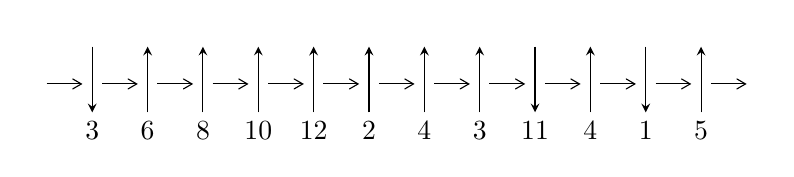
\begin{tikzpicture}[x=20pt, y=17pt]
	% nodes
	\node (C0) at (0, 0) {};
	\node (C1) at (1, 0) {};
	\node (C1U) at (1, +1) {};
	\node (C1D) at (1, -1) {3};

	\node (C2) at (2, 0) {};
	\node (C2U) at (2, +1) {};
	\node (C2D) at (2, -1) {6};

	\node (C3) at (3, 0) {};
	\node (C3U) at (3, +1) {};
	\node (C3D) at (3, -1) {8};

	\node (C4) at (4, 0) {};
	\node (C4U) at (4, +1) {};
	\node (C4D) at (4, -1) {10};

	\node (C5) at (5, 0) {};
	\node (C5U) at (5, +1) {};
	\node (C5D) at (5, -1) {12};

	\node (C6) at (6, 0) {};
	\node (C6U) at (6, +1) {};
	\node (C6D) at (6, -1) {2};

	\node (C7) at (7, 0) {};
	\node (C7U) at (7, +1) {};
	\node (C7D) at (7, -1) {4};

	\node (C8) at (8, 0) {};
	\node (C8U) at (8, +1) {};
	\node (C8D) at (8, -1) {3};

	\node (C9) at (9, 0) {};
	\node (C9U) at (9, +1) {};
	\node (C9D) at (9, -1) {11};

	\node (C10) at (10, 0) {};
	\node (C10U) at (10, +1) {};
	\node (C10D) at (10, -1) {4};

	\node (C11) at (11, 0) {};
	\node (C11U) at (11, +1) {};
	\node (C11D) at (11, -1) {1};

	\node (C12) at (12, 0) {};
	\node (C12U) at (12, +1) {};
	\node (C12D) at (12, -1) {5};
	\node (C13) at (13, 0) {};

	% arrows
	\draw[->,>={angle 60}]
	(C0) edge (C1) (C1) edge (C2) (C2) edge (C3) (C3) edge (C4) (C4) edge (C5) (C5) edge (C6) (C6) edge (C7) (C7) edge (C8) (C8) edge (C9) (C9) edge (C10) (C10) edge (C11) (C11) edge (C12) (C12) edge (C13) ;	\draw[->,>=stealth]
	(C1U) edge (C1D) (C2D) edge (C2U) (C3D) edge (C3U) (C4D) edge (C4U) (C5D) edge (C5U) (C6D) edge (C6U) (C7D) edge (C7U) (C8D) edge (C8U) (C9U) edge (C9D) (C10D) edge (C10U) (C11U) edge (C11D) (C12D) edge (C12U) ;
	\end{tikzpicture} \\
\hhline{~~} \\& 
\textbf{Solving Sequence} \\ \cline{2-2} 
 &
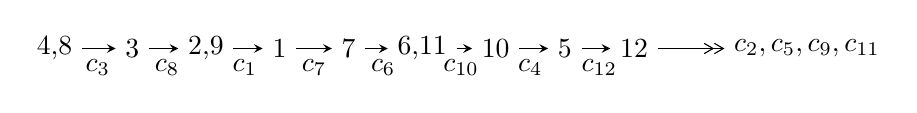
\begin{tikzpicture}[x=25pt, y=7pt]
	% node
	\node (A0) at (-1/8, 0) {4,8};
	\node (A1) at (1, 0) {3};
	\node (A2) at (33/16, 0) {2,9};
	\node (A3) at (25/8, 0) {1};
	\node (A4) at (33/8, 0) {7};
	\node (A5) at (83/16, 0) {6,11};
	\node (A6) at (25/4, 0) {10};
	\node (A7) at (29/4, 0) {5};
	\node (A8) at (33/4, 0) {12};
	\node (C1) at (1/2, -1) {$c_{3}$};
	\node (C2) at (3/2, -1) {$c_{8}$};
	\node (C3) at (21/8, -1) {$c_{1}$};
	\node (C4) at (29/8, -1) {$c_{7}$};
	\node (C5) at (37/8, -1) {$c_{6}$};
	\node (C6) at (23/4, -1) {$c_{10}$};
	\node (C7) at (27/4, -1) {$c_{4}$};
	\node (C8) at (31/4, -1) {$c_{12}$};
	\node (A9) at (43/4, 0) {$c_{2},c_{5},c_{9},c_{11}$};

	% edge
	\draw[->,>=stealth]	
	(A0) edge (A1) (A1) edge (A2) (A2) edge (A3) (A3) edge (A4) (A4) edge (A5) (A5) edge (A6) (A6) edge (A7) (A7) edge (A8) ;
	\draw[->>,>={angle 60}]	
	(A8) edge (A9);
\end{tikzpicture} \\ 

\end{tabular} \\

\footnotetext{
The image of knot diagram is generated by the software ``\textbf{Draw programme}" developed by Andrew Bartholomew(\url{http://www.layer8.co.uk/maths/draw/index.htm\#Running-draw}), where we modified some parts for our purpose(\url{https://github.com/CATsTAILs/LinksPainter}).
}\phantom \\ \newline 
\centering \textbf{Ideals for irreducible components\footnotemark of $X_{\text{par}}$} 
 
\begin{align*}
I^u_{1}&=\langle 
d- u,\;- u^4+u^3+2 c- u-1,\;u^4+u^3+2 b+u-1,\;- u^4- u^3+2 a- u-1,\;u^5+u^3+u^2+2 u-1\rangle \\
I^u_{2}&=\langle 
d- u,\;u^7+2 u^3+u^2+2 c-3 u+1,\;b+1,\;u^7+u^2+2 a-3 u+1,\;u^8- u^7+2 u^6-2 u^5+4 u^4-3 u^3+2 u^2+1\rangle \\
I^u_{3}&=\langle 
d- u,\;u^7+2 u^3+u^2+2 c-3 u+1,\;u^7-2 u^6+2 u^5-2 u^4+4 u^3-5 u^2+2 b+u-1,\\
\phantom{I^u_{3}}&\phantom{= \langle  }- u^7+2 u^6-2 u^5+2 u^4-4 u^3+5 u^2+2 a- u-1,\;u^8- u^7+2 u^6-2 u^5+4 u^4-3 u^3+2 u^2+1\rangle \\
I^u_{4}&=\langle 
- u^5-2 u^3+u^2+2 d+2,\;- u^7+u^6-3 u^5+3 u^4-3 u^3+5 u^2+4 c-4 u+4,\;b+1,\\
\phantom{I^u_{4}}&\phantom{= \langle  }- u^7+u^6-3 u^5+u^4-3 u^3+u^2+4 a-2 u,\;u^8- u^7+3 u^6-3 u^5+3 u^4-5 u^3+4 u^2-4 u+4\rangle \\
I^u_{5}&=\langle 
u^7-2 u^6+2 u^5-4 u^4+4 u^3-5 u^2+2 d+3 u-1,\;- u^7+u^6-2 u^5+2 u^4-4 u^3+3 u^2+c-2 u,\\
\phantom{I^u_{5}}&\phantom{= \langle  }u^7-2 u^6+2 u^5-2 u^4+4 u^3-5 u^2+2 b+u-1,\;- u^7+2 u^6-2 u^5+2 u^4-4 u^3+5 u^2+2 a- u-1,\\
\phantom{I^u_{5}}&\phantom{= \langle  }u^8- u^7+2 u^6-2 u^5+4 u^4-3 u^3+2 u^2+1\rangle \\
I^u_{6}&=\langle 
d- u,\;u^5- u^4+2 u^2+c- u-2,\;b+1,\;u^5+u^3+2 a+u-1,\;u^6+u^4+2 u^3+u^2+u+2\rangle \\
I^u_{7}&=\langle 
- u^3+d-1,\;- u^5- u^3-2 u^2+2 c- u-1,\;b+1,\;u^5+u^3+2 a+u-1,\;u^6+u^4+2 u^3+u^2+u+2\rangle \\
I^u_{8}&=\langle 
- u^3+d-1,\;- u^5- u^3-2 u^2+2 c- u-1,\;- u^5- u^4-2 u^2+b-3 u-2,\;u^5+u^4+2 u^2+a+3 u+1,\\
\phantom{I^u_{8}}&\phantom{= \langle  }u^6+u^4+2 u^3+u^2+u+2\rangle \\
I^u_{9}&=\langle 
d- u,\;c+2,\;b+1,\;a^2- a+u+1,\;u^2+u+1\rangle \\
I^u_{10}&=\langle 
- u^3+d- u+1,\;- u^3+u^2+c-2 u+2,\;b+1,\;- u^3+a-2 u,\;u^4- u^3+2 u^2-2 u+1\rangle \\
\end{align*}\\
\begin{align*}
I^u_{11}&=\langle 
- u^3+d- u+1,\;- u^3+u^2+c-2 u+2,\;b+1,\;u^3+a+2 u-1,\;u^4- u^3+2 u^2-2 u+1\rangle \\
I^u_{12}&=\langle 
u^3+d+2 u-1,\;- u^3+u^2+c-2 u+2,\;b+1,\;- u^3+a-2 u,\;u^4- u^3+2 u^2-2 u+1\rangle \\
I^u_{13}&=\langle 
a u+d,\;c- u-1,\;b+1,\;a^2- a+u+1,\;u^2+u+1\rangle \\
I^u_{14}&=\langle 
d^2+d u- u,\;c- u-1,\;b+2 u,\;a-2 u-1,\;u^2+u+1\rangle \\
I^u_{15}&=\langle 
d,\;c- u,\;b+u+1,\;a- u,\;u^2+1\rangle \\
I^u_{16}&=\langle 
d+u,\;c- u+1,\;b+1,\;a-1,\;u^2+1\rangle \\
I^u_{17}&=\langle 
d+u,\;c- u+1,\;b+u+1,\;a- u,\;u^2+1\rangle \\
I^u_{18}&=\langle 
d+u,\;c a- a u+u+1,\;b+a+1,\;u^2+1\rangle \\
\\
I^v_{1}&=\langle 
a,\;d+v,\;- a v+c+v+1,\;b+1,\;v^2+1\rangle \\
\end{align*}
\raggedright * 18 irreducible components of $\dim_{\mathbb{C}}=0$, with total 87 representations.\\
\raggedright * 1 irreducible components of $\dim_{\mathbb{C}}=1$ \\
\footnotetext{All coefficients of polynomials are rational numbers. But the coefficients are sometimes approximated in decimal forms when there is not enough margin.}
\newpage
\renewcommand{\arraystretch}{1}
\centering \section*{I. $I^u_{1}= \langle d- u,\;- u^4+u^3+2 c- u-1,\;u^4+u^3+2 b+u-1,\;- u^4- u^3+2 a- u-1,\;u^5+u^3+u^2+2 u-1 \rangle$}
\flushleft \textbf{(i) Arc colorings}\\
\begin{tabular}{m{7pt} m{180pt} m{7pt} m{180pt} }
\flushright $a_{4}=$&$\begin{pmatrix}1\\0\end{pmatrix}$ \\
\flushright $a_{8}=$&$\begin{pmatrix}0\\u\end{pmatrix}$ \\
\flushright $a_{3}=$&$\begin{pmatrix}1\\u^2\end{pmatrix}$ \\
\flushright $a_{2}=$&$\begin{pmatrix}\frac{1}{2} u^4+\frac{1}{2} u^3+\frac{1}{2} u+\frac{1}{2}\\-\frac{1}{2} u^4-\frac{1}{2} u^3-\frac{1}{2} u+\frac{1}{2}\end{pmatrix}$ \\
\flushright $a_{9}=$&$\begin{pmatrix}u\\u^3+u\end{pmatrix}$ \\
\flushright $a_{1}=$&$\begin{pmatrix}\frac{1}{2} u^4+\frac{1}{2} u^3+u^2+\frac{1}{2} u+\frac{1}{2}\\\frac{1}{2} u^4-\frac{1}{2} u^3-\frac{1}{2} u+\frac{1}{2}\end{pmatrix}$ \\
\flushright $a_{7}=$&$\begin{pmatrix}- u\\u\end{pmatrix}$ \\
\flushright $a_{6}=$&$\begin{pmatrix}-\frac{1}{2} u^4+\frac{1}{2} u^3-\frac{1}{2} u-\frac{1}{2}\\\frac{1}{2} u^4-\frac{1}{2} u^3-\frac{1}{2} u+\frac{1}{2}\end{pmatrix}$ \\
\flushright $a_{11}=$&$\begin{pmatrix}\frac{1}{2} u^4-\frac{1}{2} u^3+\frac{1}{2} u+\frac{1}{2}\\u\end{pmatrix}$ \\
\flushright $a_{10}=$&$\begin{pmatrix}\frac{1}{2} u^4-\frac{1}{2} u^3-\frac{1}{2} u+\frac{1}{2}\\u\end{pmatrix}$ \\
\flushright $a_{5}=$&$\begin{pmatrix}\frac{1}{2} u^4+\frac{1}{2} u^3+u^2+\frac{1}{2} u+\frac{1}{2}\\- u^2\end{pmatrix}$ \\
\flushright $a_{12}=$&$\begin{pmatrix}u^2+u\\\frac{1}{2} u^4+\frac{1}{2} u^3-\frac{1}{2} u+\frac{1}{2}\end{pmatrix}$\\&\end{tabular}
\flushleft \textbf{(ii) Obstruction class $= -1$}\\~\\
\flushleft \textbf{(iii) Cusp Shapes $= 4 u^4+4 u^3+4 u+14$}\\~\\
\newpage\renewcommand{\arraystretch}{1}
\flushleft \textbf{(iv) u-Polynomials at the component}\newline \\
\begin{tabular}{m{50pt}|m{274pt}}
Crossings & \hspace{64pt}u-Polynomials at each crossing \\
\hline $$\begin{aligned}c_{1},c_{9},c_{11}\end{aligned}$$&$\begin{aligned}
&u^5+2 u^4+5 u^3+3 u^2+6 u-1
\end{aligned}$\\
\hline $$\begin{aligned}c_{2},c_{3},c_{4}\\c_{5},c_{6},c_{7}\\c_{8},c_{10},c_{12}\end{aligned}$$&$\begin{aligned}
&u^5+u^3+u^2+2 u-1
\end{aligned}$\\
\hline
\end{tabular}\\~\\
\newpage\renewcommand{\arraystretch}{1}
\flushleft \textbf{(v) Riley Polynomials at the component}\newline \\
\begin{tabular}{m{50pt}|m{274pt}}
Crossings & \hspace{64pt}Riley Polynomials at each crossing \\
\hline $$\begin{aligned}c_{1},c_{9},c_{11}\end{aligned}$$&$\begin{aligned}
&y^5+6 y^4+25 y^3+55 y^2+42 y-1
\end{aligned}$\\
\hline $$\begin{aligned}c_{2},c_{3},c_{4}\\c_{5},c_{6},c_{7}\\c_{8},c_{10},c_{12}\end{aligned}$$&$\begin{aligned}
&y^5+2 y^4+5 y^3+3 y^2+6 y-1
\end{aligned}$\\
\hline
\end{tabular}\\~\\
\newpage\flushleft \textbf{(vi) Complex Volumes and Cusp Shapes}
$$\begin{array}{c|c|c}  
\text{Solutions to }I^u_{1}& \I (\text{vol} + \sqrt{-1}CS) & \text{Cusp shape}\\
 \hline 
\begin{aligned}
u &= -0.828442 + 0.812698 I \\
a &= -0.284015 + 0.939824 I \\
b &= \phantom{-}1.28401 - 0.93982 I \\
c &= -1.356950 - 0.196710 I \\
d &= -0.828442 + 0.812698 I\end{aligned}
 & \phantom{-}4.34615 - 6.57943 I & \phantom{-}7.72788 + 7.51859 I \\ \hline\begin{aligned}
u &= -0.828442 - 0.812698 I \\
a &= -0.284015 - 0.939824 I \\
b &= \phantom{-}1.28401 + 0.93982 I \\
c &= -1.356950 + 0.196710 I \\
d &= -0.828442 - 0.812698 I\end{aligned}
 & \phantom{-}4.34615 + 6.57943 I & \phantom{-}7.72788 - 7.51859 I \\ \hline\begin{aligned}
u &= \phantom{-}0.633508 + 1.226040 I \\
a &= -1.08404 - 1.28198 I \\
b &= \phantom{-}2.08404 + 1.28198 I \\
c &= \phantom{-}1.51852 - 0.91518 I \\
d &= \phantom{-}0.633508 + 1.226040 I\end{aligned}
 & -2.1892 + 16.8691 I & \phantom{-}1.32766 - 10.25585 I \\ \hline\begin{aligned}
u &= \phantom{-}0.633508 - 1.226040 I \\
a &= -1.08404 + 1.28198 I \\
b &= \phantom{-}2.08404 - 1.28198 I \\
c &= \phantom{-}1.51852 + 0.91518 I \\
d &= \phantom{-}0.633508 - 1.226040 I\end{aligned}
 & -2.1892 - 16.8691 I & \phantom{-}1.32766 + 10.25585 I \\ \hline\begin{aligned}
u &= \phantom{-}0.389868\phantom{ +0.000000I} \\
a &= \phantom{-}0.736115\phantom{ +0.000000I} \\
b &= \phantom{-}0.263885\phantom{ +0.000000I} \\
c &= \phantom{-}0.676856\phantom{ +0.000000I} \\
d &= \phantom{-}0.389868\phantom{ +0.000000I}\end{aligned}
 & \phantom{-}0.620982\phantom{ +0.000000I} & \phantom{-}15.8890\phantom{ +0.000000I}\\
 \hline 
 \end{array}$$\newpage\newpage\renewcommand{\arraystretch}{1}
\centering \section*{II. $I^u_{2}= \langle d- u,\;u^7+2 u^3+\cdots+2 c+1,\;b+1,\;u^7+u^2+2 a-3 u+1,\;u^8- u^7+\cdots+2 u^2+1 \rangle$}
\flushleft \textbf{(i) Arc colorings}\\
\begin{tabular}{m{7pt} m{180pt} m{7pt} m{180pt} }
\flushright $a_{4}=$&$\begin{pmatrix}1\\0\end{pmatrix}$ \\
\flushright $a_{8}=$&$\begin{pmatrix}0\\u\end{pmatrix}$ \\
\flushright $a_{3}=$&$\begin{pmatrix}1\\u^2\end{pmatrix}$ \\
\flushright $a_{2}=$&$\begin{pmatrix}-\frac{1}{2} u^7-\frac{1}{2} u^2+\frac{3}{2} u-\frac{1}{2}\\-1\end{pmatrix}$ \\
\flushright $a_{9}=$&$\begin{pmatrix}u\\u^3+u\end{pmatrix}$ \\
\flushright $a_{1}=$&$\begin{pmatrix}- u^7- u^5- u^3- u^2+u-2\\-\frac{1}{2} u^7- u^3-\frac{1}{2} u^2+\frac{1}{2} u-\frac{1}{2}\end{pmatrix}$ \\
\flushright $a_{7}=$&$\begin{pmatrix}- u\\u\end{pmatrix}$ \\
\flushright $a_{6}=$&$\begin{pmatrix}- u^7+u^6-2 u^5+2 u^4-4 u^3+3 u^2-2 u\\-\frac{1}{2} u^7+u^6+\cdots-\frac{1}{2} u+\frac{1}{2}\end{pmatrix}$ \\
\flushright $a_{11}=$&$\begin{pmatrix}-\frac{1}{2} u^7- u^3-\frac{1}{2} u^2+\frac{3}{2} u-\frac{1}{2}\\u\end{pmatrix}$ \\
\flushright $a_{10}=$&$\begin{pmatrix}-\frac{1}{2} u^7- u^3-\frac{1}{2} u^2+\frac{1}{2} u-\frac{1}{2}\\u\end{pmatrix}$ \\
\flushright $a_{5}=$&$\begin{pmatrix}\frac{1}{2} u^7- u^6+\cdots+\frac{1}{2} u+\frac{1}{2}\\- u^2\end{pmatrix}$ \\
\flushright $a_{12}=$&$\begin{pmatrix}-\frac{1}{2} u^7- u^5+\cdots+\frac{1}{2} u-\frac{3}{2}\\-\frac{1}{2} u^7-\frac{1}{2} u^2+\frac{1}{2} u-\frac{1}{2}\end{pmatrix}$\\&\end{tabular}
\flushleft \textbf{(ii) Obstruction class $= -1$}\\~\\
\flushleft \textbf{(iii) Cusp Shapes $= -4 u^6+2 u^5-4 u^4+6 u^3-12 u^2+6 u+4$}\\~\\
\newpage\renewcommand{\arraystretch}{1}
\flushleft \textbf{(iv) u-Polynomials at the component}\newline \\
\begin{tabular}{m{50pt}|m{274pt}}
Crossings & \hspace{64pt}u-Polynomials at each crossing \\
\hline $$\begin{aligned}c_{1}\end{aligned}$$&$\begin{aligned}
&u^8+5 u^7+9 u^6+7 u^5+3 u^4- u^3+16 u+16
\end{aligned}$\\
\hline $$\begin{aligned}c_{2},c_{6}\end{aligned}$$&$\begin{aligned}
&u^8- u^7+3 u^6-3 u^5+3 u^4-5 u^3+4 u^2-4 u+4
\end{aligned}$\\
\hline $$\begin{aligned}c_{3},c_{4},c_{5}\\c_{7},c_{8},c_{10}\\c_{12}\end{aligned}$$&$\begin{aligned}
&u^8- u^7+2 u^6-2 u^5+4 u^4-3 u^3+2 u^2+1
\end{aligned}$\\
\hline $$\begin{aligned}c_{9},c_{11}\end{aligned}$$&$\begin{aligned}
&u^8+3 u^7+8 u^6+10 u^5+14 u^4+11 u^3+12 u^2+4 u+1
\end{aligned}$\\
\hline
\end{tabular}\\~\\
\newpage\renewcommand{\arraystretch}{1}
\flushleft \textbf{(v) Riley Polynomials at the component}\newline \\
\begin{tabular}{m{50pt}|m{274pt}}
Crossings & \hspace{64pt}Riley Polynomials at each crossing \\
\hline $$\begin{aligned}c_{1}\end{aligned}$$&$\begin{aligned}
&y^8-7 y^7+17 y^6+15 y^5-105 y^4+63 y^3+128 y^2-256 y+256
\end{aligned}$\\
\hline $$\begin{aligned}c_{2},c_{6}\end{aligned}$$&$\begin{aligned}
&y^8+5 y^7+9 y^6+7 y^5+3 y^4- y^3+16 y+16
\end{aligned}$\\
\hline $$\begin{aligned}c_{3},c_{4},c_{5}\\c_{7},c_{8},c_{10}\\c_{12}\end{aligned}$$&$\begin{aligned}
&y^8+3 y^7+8 y^6+10 y^5+14 y^4+11 y^3+12 y^2+4 y+1
\end{aligned}$\\
\hline $$\begin{aligned}c_{9},c_{11}\end{aligned}$$&$\begin{aligned}
&y^8+7 y^7+32 y^6+82 y^5+146 y^4+151 y^3+84 y^2+8 y+1
\end{aligned}$\\
\hline
\end{tabular}\\~\\
\newpage\flushleft \textbf{(vi) Complex Volumes and Cusp Shapes}
$$\begin{array}{c|c|c}  
\text{Solutions to }I^u_{2}& \I (\text{vol} + \sqrt{-1}CS) & \text{Cusp shape}\\
 \hline 
\begin{aligned}
u &= \phantom{-}0.862697 + 0.615401 I \\
a &= \phantom{-}0.886105 + 1.090380 I \\
b &= -1.00000\phantom{ +0.000000I} \\
c &= \phantom{-}1.224210 - 0.050581 I \\
d &= \phantom{-}0.862697 + 0.615401 I\end{aligned}
 & \phantom{-}4.15083 + 0.66722 I & \phantom{-}8.81639 - 2.10627 I \\ \hline\begin{aligned}
u &= \phantom{-}0.862697 - 0.615401 I \\
a &= \phantom{-}0.886105 - 1.090380 I \\
b &= -1.00000\phantom{ +0.000000I} \\
c &= \phantom{-}1.224210 + 0.050581 I \\
d &= \phantom{-}0.862697 - 0.615401 I\end{aligned}
 & \phantom{-}4.15083 - 0.66722 I & \phantom{-}8.81639 + 2.10627 I \\ \hline\begin{aligned}
u &= \phantom{-}0.578102 + 1.055330 I \\
a &= \phantom{-}0.102567 - 0.732209 I \\
b &= -1.00000\phantom{ +0.000000I} \\
c &= \phantom{-}1.84091 - 0.61494 I \\
d &= \phantom{-}0.578102 + 1.055330 I\end{aligned}
 & -5.02390 + 6.79402 I & \phantom{-}0.88161 - 7.09473 I \\ \hline\begin{aligned}
u &= \phantom{-}0.578102 - 1.055330 I \\
a &= \phantom{-}0.102567 + 0.732209 I \\
b &= -1.00000\phantom{ +0.000000I} \\
c &= \phantom{-}1.84091 + 0.61494 I \\
d &= \phantom{-}0.578102 - 1.055330 I\end{aligned}
 & -5.02390 - 6.79402 I & \phantom{-}0.88161 + 7.09473 I \\ \hline\begin{aligned}
u &= -0.666851 + 1.155530 I \\
a &= \phantom{-}0.821510 - 0.756488 I \\
b &= -1.00000\phantom{ +0.000000I} \\
c &= -1.55320 - 0.75511 I \\
d &= -0.666851 + 1.155530 I\end{aligned}
 & \phantom{-}0.65207 - 10.98940 I & \phantom{-}4.47099 + 7.14773 I \\ \hline\begin{aligned}
u &= -0.666851 - 1.155530 I \\
a &= \phantom{-}0.821510 + 0.756488 I \\
b &= -1.00000\phantom{ +0.000000I} \\
c &= -1.55320 + 0.75511 I \\
d &= -0.666851 - 1.155530 I\end{aligned}
 & \phantom{-}0.65207 + 10.98940 I & \phantom{-}4.47099 - 7.14773 I\\
 \hline 
 \end{array}$$\newpage$$\begin{array}{c|c|c}  
\text{Solutions to }I^u_{2}& \I (\text{vol} + \sqrt{-1}CS) & \text{Cusp shape}\\
 \hline 
\begin{aligned}
u &= -0.273948 + 0.520074 I \\
a &= -0.810182 + 0.910843 I \\
b &= -1.00000\phantom{ +0.000000I} \\
c &= -1.011910 + 0.934421 I \\
d &= -0.273948 + 0.520074 I\end{aligned}
 & -3.06886 - 1.27680 I & \phantom{-}5.83102 + 5.88514 I \\ \hline\begin{aligned}
u &= -0.273948 - 0.520074 I \\
a &= -0.810182 - 0.910843 I \\
b &= -1.00000\phantom{ +0.000000I} \\
c &= -1.011910 - 0.934421 I \\
d &= -0.273948 - 0.520074 I\end{aligned}
 & -3.06886 + 1.27680 I & \phantom{-}5.83102 - 5.88514 I\\
 \hline 
 \end{array}$$\newpage\newpage\renewcommand{\arraystretch}{1}
\centering \section*{III. $I^u_{3}= \langle d- u,\;u^7+2 u^3+\cdots+2 c+1,\;u^7-2 u^6+\cdots+2 b-1,\;- u^7+2 u^6+\cdots+2 a-1,\;u^8- u^7+\cdots+2 u^2+1 \rangle$}
\flushleft \textbf{(i) Arc colorings}\\
\begin{tabular}{m{7pt} m{180pt} m{7pt} m{180pt} }
\flushright $a_{4}=$&$\begin{pmatrix}1\\0\end{pmatrix}$ \\
\flushright $a_{8}=$&$\begin{pmatrix}0\\u\end{pmatrix}$ \\
\flushright $a_{3}=$&$\begin{pmatrix}1\\u^2\end{pmatrix}$ \\
\flushright $a_{2}=$&$\begin{pmatrix}\frac{1}{2} u^7- u^6+\cdots+\frac{1}{2} u+\frac{1}{2}\\-\frac{1}{2} u^7+u^6+\cdots-\frac{1}{2} u+\frac{1}{2}\end{pmatrix}$ \\
\flushright $a_{9}=$&$\begin{pmatrix}u\\u^3+u\end{pmatrix}$ \\
\flushright $a_{1}=$&$\begin{pmatrix}\frac{1}{2} u^7- u^6+\cdots+\frac{1}{2} u+\frac{1}{2}\\-\frac{1}{2} u^7+u^6+\cdots-\frac{1}{2} u+\frac{1}{2}\end{pmatrix}$ \\
\flushright $a_{7}=$&$\begin{pmatrix}- u\\u\end{pmatrix}$ \\
\flushright $a_{6}=$&$\begin{pmatrix}\frac{1}{2} u^7+u^3+\frac{1}{2} u^2-\frac{3}{2} u+\frac{1}{2}\\-\frac{1}{2} u^7- u^3-\frac{1}{2} u^2+\frac{1}{2} u-\frac{1}{2}\end{pmatrix}$ \\
\flushright $a_{11}=$&$\begin{pmatrix}-\frac{1}{2} u^7- u^3-\frac{1}{2} u^2+\frac{3}{2} u-\frac{1}{2}\\u\end{pmatrix}$ \\
\flushright $a_{10}=$&$\begin{pmatrix}-\frac{1}{2} u^7- u^3-\frac{1}{2} u^2+\frac{1}{2} u-\frac{1}{2}\\u\end{pmatrix}$ \\
\flushright $a_{5}=$&$\begin{pmatrix}\frac{1}{2} u^7- u^6+\cdots+\frac{1}{2} u+\frac{1}{2}\\- u^2\end{pmatrix}$ \\
\flushright $a_{12}=$&$\begin{pmatrix}- u^6+u^5- u^4+2 u^3-3 u^2+2 u\\u^6+u^4- u^3+2 u^2\end{pmatrix}$\\&\end{tabular}
\flushleft \textbf{(ii) Obstruction class $= -1$}\\~\\
\flushleft \textbf{(iii) Cusp Shapes $= -4 u^6+2 u^5-4 u^4+6 u^3-12 u^2+6 u+4$}\\~\\
\newpage\renewcommand{\arraystretch}{1}
\flushleft \textbf{(iv) u-Polynomials at the component}\newline \\
\begin{tabular}{m{50pt}|m{274pt}}
Crossings & \hspace{64pt}u-Polynomials at each crossing \\
\hline $$\begin{aligned}c_{1},c_{9}\end{aligned}$$&$\begin{aligned}
&u^8+3 u^7+8 u^6+10 u^5+14 u^4+11 u^3+12 u^2+4 u+1
\end{aligned}$\\
\hline $$\begin{aligned}c_{2},c_{3},c_{4}\\c_{6},c_{7},c_{8}\\c_{10}\end{aligned}$$&$\begin{aligned}
&u^8- u^7+2 u^6-2 u^5+4 u^4-3 u^3+2 u^2+1
\end{aligned}$\\
\hline $$\begin{aligned}c_{5},c_{12}\end{aligned}$$&$\begin{aligned}
&u^8- u^7+3 u^6-3 u^5+3 u^4-5 u^3+4 u^2-4 u+4
\end{aligned}$\\
\hline $$\begin{aligned}c_{11}\end{aligned}$$&$\begin{aligned}
&u^8+5 u^7+9 u^6+7 u^5+3 u^4- u^3+16 u+16
\end{aligned}$\\
\hline
\end{tabular}\\~\\
\newpage\renewcommand{\arraystretch}{1}
\flushleft \textbf{(v) Riley Polynomials at the component}\newline \\
\begin{tabular}{m{50pt}|m{274pt}}
Crossings & \hspace{64pt}Riley Polynomials at each crossing \\
\hline $$\begin{aligned}c_{1},c_{9}\end{aligned}$$&$\begin{aligned}
&y^8+7 y^7+32 y^6+82 y^5+146 y^4+151 y^3+84 y^2+8 y+1
\end{aligned}$\\
\hline $$\begin{aligned}c_{2},c_{3},c_{4}\\c_{6},c_{7},c_{8}\\c_{10}\end{aligned}$$&$\begin{aligned}
&y^8+3 y^7+8 y^6+10 y^5+14 y^4+11 y^3+12 y^2+4 y+1
\end{aligned}$\\
\hline $$\begin{aligned}c_{5},c_{12}\end{aligned}$$&$\begin{aligned}
&y^8+5 y^7+9 y^6+7 y^5+3 y^4- y^3+16 y+16
\end{aligned}$\\
\hline $$\begin{aligned}c_{11}\end{aligned}$$&$\begin{aligned}
&y^8-7 y^7+17 y^6+15 y^5-105 y^4+63 y^3+128 y^2-256 y+256
\end{aligned}$\\
\hline
\end{tabular}\\~\\
\newpage\flushleft \textbf{(vi) Complex Volumes and Cusp Shapes}
$$\begin{array}{c|c|c}  
\text{Solutions to }I^u_{3}& \I (\text{vol} + \sqrt{-1}CS) & \text{Cusp shape}\\
 \hline 
\begin{aligned}
u &= \phantom{-}0.862697 + 0.615401 I \\
a &= -0.087246 - 0.709742 I \\
b &= \phantom{-}1.087250 + 0.709742 I \\
c &= \phantom{-}1.224210 - 0.050581 I \\
d &= \phantom{-}0.862697 + 0.615401 I\end{aligned}
 & \phantom{-}4.15083 + 0.66722 I & \phantom{-}8.81639 - 2.10627 I \\ \hline\begin{aligned}
u &= \phantom{-}0.862697 - 0.615401 I \\
a &= -0.087246 + 0.709742 I \\
b &= \phantom{-}1.087250 - 0.709742 I \\
c &= \phantom{-}1.224210 + 0.050581 I \\
d &= \phantom{-}0.862697 - 0.615401 I\end{aligned}
 & \phantom{-}4.15083 - 0.66722 I & \phantom{-}8.81639 + 2.10627 I \\ \hline\begin{aligned}
u &= \phantom{-}0.578102 + 1.055330 I \\
a &= -0.71320 - 1.58728 I \\
b &= \phantom{-}1.71320 + 1.58728 I \\
c &= \phantom{-}1.84091 - 0.61494 I \\
d &= \phantom{-}0.578102 + 1.055330 I\end{aligned}
 & -5.02390 + 6.79402 I & \phantom{-}0.88161 - 7.09473 I \\ \hline\begin{aligned}
u &= \phantom{-}0.578102 - 1.055330 I \\
a &= -0.71320 + 1.58728 I \\
b &= \phantom{-}1.71320 - 1.58728 I \\
c &= \phantom{-}1.84091 + 0.61494 I \\
d &= \phantom{-}0.578102 - 1.055330 I\end{aligned}
 & -5.02390 - 6.79402 I & \phantom{-}0.88161 + 7.09473 I \\ \hline\begin{aligned}
u &= -0.666851 + 1.155530 I \\
a &= -0.90831 + 1.29123 I \\
b &= \phantom{-}1.90831 - 1.29123 I \\
c &= -1.55320 - 0.75511 I \\
d &= -0.666851 + 1.155530 I\end{aligned}
 & \phantom{-}0.65207 - 10.98940 I & \phantom{-}4.47099 + 7.14773 I \\ \hline\begin{aligned}
u &= -0.666851 - 1.155530 I \\
a &= -0.90831 - 1.29123 I \\
b &= \phantom{-}1.90831 + 1.29123 I \\
c &= -1.55320 + 0.75511 I \\
d &= -0.666851 - 1.155530 I\end{aligned}
 & \phantom{-}0.65207 + 10.98940 I & \phantom{-}4.47099 - 7.14773 I\\
 \hline 
 \end{array}$$\newpage$$\begin{array}{c|c|c}  
\text{Solutions to }I^u_{3}& \I (\text{vol} + \sqrt{-1}CS) & \text{Cusp shape}\\
 \hline 
\begin{aligned}
u &= -0.273948 + 0.520074 I \\
a &= \phantom{-}1.20876 + 0.78225 I \\
b &= -0.208757 - 0.782252 I \\
c &= -1.011910 + 0.934421 I \\
d &= -0.273948 + 0.520074 I\end{aligned}
 & -3.06886 - 1.27680 I & \phantom{-}5.83102 + 5.88514 I \\ \hline\begin{aligned}
u &= -0.273948 - 0.520074 I \\
a &= \phantom{-}1.20876 - 0.78225 I \\
b &= -0.208757 + 0.782252 I \\
c &= -1.011910 - 0.934421 I \\
d &= -0.273948 - 0.520074 I\end{aligned}
 & -3.06886 + 1.27680 I & \phantom{-}5.83102 - 5.88514 I\\
 \hline 
 \end{array}$$\newpage\newpage\renewcommand{\arraystretch}{1}
\centering \section*{IV. $I^u_{4}= \langle - u^5-2 u^3+u^2+2 d+2,\;- u^7+u^6+\cdots+4 c+4,\;b+1,\;- u^7+u^6+\cdots+4 a-2 u,\;u^8- u^7+\cdots-4 u+4 \rangle$}
\flushleft \textbf{(i) Arc colorings}\\
\begin{tabular}{m{7pt} m{180pt} m{7pt} m{180pt} }
\flushright $a_{4}=$&$\begin{pmatrix}1\\0\end{pmatrix}$ \\
\flushright $a_{8}=$&$\begin{pmatrix}0\\u\end{pmatrix}$ \\
\flushright $a_{3}=$&$\begin{pmatrix}1\\u^2\end{pmatrix}$ \\
\flushright $a_{2}=$&$\begin{pmatrix}\frac{1}{4} u^7-\frac{1}{4} u^6+\cdots-\frac{1}{4} u^2+\frac{1}{2} u\\-1\end{pmatrix}$ \\
\flushright $a_{9}=$&$\begin{pmatrix}u\\u^3+u\end{pmatrix}$ \\
\flushright $a_{1}=$&$\begin{pmatrix}\frac{1}{4} u^7-\frac{3}{4} u^6+\cdots+\frac{3}{2} u-1\\-\frac{1}{2} u^7+\frac{1}{2} u^6+\cdots-2 u+1\end{pmatrix}$ \\
\flushright $a_{7}=$&$\begin{pmatrix}- u\\u\end{pmatrix}$ \\
\flushright $a_{6}=$&$\begin{pmatrix}-\frac{1}{4} u^7+\frac{1}{4} u^6+\cdots- u+1\\\frac{1}{2} u^5+u^3-\frac{1}{2} u^2+u-1\end{pmatrix}$ \\
\flushright $a_{11}=$&$\begin{pmatrix}\frac{1}{4} u^7-\frac{1}{4} u^6+\cdots+u-1\\\frac{1}{2} u^5+u^3-\frac{1}{2} u^2-1\end{pmatrix}$ \\
\flushright $a_{10}=$&$\begin{pmatrix}\frac{1}{4} u^7-\frac{1}{4} u^6+\cdots-\frac{3}{4} u^2+u\\\frac{1}{2} u^5+u^3-\frac{1}{2} u^2-1\end{pmatrix}$ \\
\flushright $a_{5}=$&$\begin{pmatrix}\frac{1}{4} u^7-\frac{3}{4} u^6+\cdots+\frac{3}{2} u-1\\\frac{1}{2} u^6+u^4-\frac{1}{2} u^3+u^2- u+1\end{pmatrix}$ \\
\flushright $a_{12}=$&$\begin{pmatrix}-\frac{1}{2} u^6+\frac{1}{2} u^5+\cdots+\frac{1}{2} u-1\\-\frac{1}{2} u^7+\frac{1}{2} u^6+\cdots- u+2\end{pmatrix}$\\&\end{tabular}
\flushleft \textbf{(ii) Obstruction class $= -1$}\\~\\
\flushleft \textbf{(iii) Cusp Shapes $= u^7+3 u^6+u^5+3 u^4- u^3+u^2-6 u+10$}\\~\\
\newpage\renewcommand{\arraystretch}{1}
\flushleft \textbf{(iv) u-Polynomials at the component}\newline \\
\begin{tabular}{m{50pt}|m{274pt}}
Crossings & \hspace{64pt}u-Polynomials at each crossing \\
\hline $$\begin{aligned}c_{1},c_{9},c_{11}\end{aligned}$$&$\begin{aligned}
&u^8+3 u^7+8 u^6+10 u^5+14 u^4+11 u^3+12 u^2+4 u+1
\end{aligned}$\\
\hline $$\begin{aligned}c_{2},c_{4},c_{5}\\c_{6},c_{10},c_{12}\end{aligned}$$&$\begin{aligned}
&u^8- u^7+2 u^6-2 u^5+4 u^4-3 u^3+2 u^2+1
\end{aligned}$\\
\hline $$\begin{aligned}c_{3},c_{7},c_{8}\end{aligned}$$&$\begin{aligned}
&u^8- u^7+3 u^6-3 u^5+3 u^4-5 u^3+4 u^2-4 u+4
\end{aligned}$\\
\hline
\end{tabular}\\~\\
\newpage\renewcommand{\arraystretch}{1}
\flushleft \textbf{(v) Riley Polynomials at the component}\newline \\
\begin{tabular}{m{50pt}|m{274pt}}
Crossings & \hspace{64pt}Riley Polynomials at each crossing \\
\hline $$\begin{aligned}c_{1},c_{9},c_{11}\end{aligned}$$&$\begin{aligned}
&y^8+7 y^7+32 y^6+82 y^5+146 y^4+151 y^3+84 y^2+8 y+1
\end{aligned}$\\
\hline $$\begin{aligned}c_{2},c_{4},c_{5}\\c_{6},c_{10},c_{12}\end{aligned}$$&$\begin{aligned}
&y^8+3 y^7+8 y^6+10 y^5+14 y^4+11 y^3+12 y^2+4 y+1
\end{aligned}$\\
\hline $$\begin{aligned}c_{3},c_{7},c_{8}\end{aligned}$$&$\begin{aligned}
&y^8+5 y^7+9 y^6+7 y^5+3 y^4- y^3+16 y+16
\end{aligned}$\\
\hline
\end{tabular}\\~\\
\newpage\flushleft \textbf{(vi) Complex Volumes and Cusp Shapes}
$$\begin{array}{c|c|c}  
\text{Solutions to }I^u_{4}& \I (\text{vol} + \sqrt{-1}CS) & \text{Cusp shape}\\
 \hline 
\begin{aligned}
u &= \phantom{-}0.993174 + 0.298213 I \\
a &= \phantom{-}0.70455 + 1.25219 I \\
b &= -1.00000\phantom{ +0.000000I} \\
c &= -0.923603 + 0.277324 I \\
d &= -0.666851 + 1.155530 I\end{aligned}
 & \phantom{-}0.65207 - 10.98940 I & \phantom{-}4.47099 + 7.14773 I \\ \hline\begin{aligned}
u &= \phantom{-}0.993174 - 0.298213 I \\
a &= \phantom{-}0.70455 - 1.25219 I \\
b &= -1.00000\phantom{ +0.000000I} \\
c &= -0.923603 - 0.277324 I \\
d &= -0.666851 - 1.155530 I\end{aligned}
 & \phantom{-}0.65207 + 10.98940 I & \phantom{-}4.47099 - 7.14773 I \\ \hline\begin{aligned}
u &= -0.769280 + 0.870579 I \\
a &= \phantom{-}0.905238 - 0.907210 I \\
b &= -1.00000\phantom{ +0.000000I} \\
c &= \phantom{-}0.569964 + 0.645017 I \\
d &= \phantom{-}0.862697 + 0.615401 I\end{aligned}
 & \phantom{-}4.15083 + 0.66722 I & \phantom{-}8.81639 - 2.10627 I \\ \hline\begin{aligned}
u &= -0.769280 - 0.870579 I \\
a &= \phantom{-}0.905238 + 0.907210 I \\
b &= -1.00000\phantom{ +0.000000I} \\
c &= \phantom{-}0.569964 - 0.645017 I \\
d &= \phantom{-}0.862697 - 0.615401 I\end{aligned}
 & \phantom{-}4.15083 - 0.66722 I & \phantom{-}8.81639 + 2.10627 I \\ \hline\begin{aligned}
u &= \phantom{-}0.022189 + 1.190950 I \\
a &= \phantom{-}0.559180 + 0.221811 I \\
b &= -1.00000\phantom{ +0.000000I} \\
c &= -0.015639 + 0.839373 I \\
d &= -0.273948 - 0.520074 I\end{aligned}
 & -3.06886 + 1.27680 I & \phantom{-}5.83102 - 5.88514 I \\ \hline\begin{aligned}
u &= \phantom{-}0.022189 - 1.190950 I \\
a &= \phantom{-}0.559180 - 0.221811 I \\
b &= -1.00000\phantom{ +0.000000I} \\
c &= -0.015639 - 0.839373 I \\
d &= -0.273948 + 0.520074 I\end{aligned}
 & -3.06886 - 1.27680 I & \phantom{-}5.83102 + 5.88514 I\\
 \hline 
 \end{array}$$\newpage$$\begin{array}{c|c|c}  
\text{Solutions to }I^u_{4}& \I (\text{vol} + \sqrt{-1}CS) & \text{Cusp shape}\\
 \hline 
\begin{aligned}
u &= \phantom{-}0.253917 + 1.370380 I \\
a &= \phantom{-}0.331031 - 0.545807 I \\
b &= -1.00000\phantom{ +0.000000I} \\
c &= -0.130722 + 0.705502 I \\
d &= \phantom{-}0.578102 - 1.055330 I\end{aligned}
 & -5.02390 - 6.79402 I & \phantom{-}0.88161 + 7.09473 I \\ \hline\begin{aligned}
u &= \phantom{-}0.253917 - 1.370380 I \\
a &= \phantom{-}0.331031 + 0.545807 I \\
b &= -1.00000\phantom{ +0.000000I} \\
c &= -0.130722 - 0.705502 I \\
d &= \phantom{-}0.578102 + 1.055330 I\end{aligned}
 & -5.02390 + 6.79402 I & \phantom{-}0.88161 - 7.09473 I\\
 \hline 
 \end{array}$$\newpage\newpage\renewcommand{\arraystretch}{1}
\centering \section*{V. $I^u_{5}= \langle u^7-2 u^6+\cdots+2 d-1,\;- u^7+u^6+\cdots+c-2 u,\;u^7-2 u^6+\cdots+2 b-1,\;- u^7+2 u^6+\cdots+2 a-1,\;u^8- u^7+\cdots+2 u^2+1 \rangle$}
\flushleft \textbf{(i) Arc colorings}\\
\begin{tabular}{m{7pt} m{180pt} m{7pt} m{180pt} }
\flushright $a_{4}=$&$\begin{pmatrix}1\\0\end{pmatrix}$ \\
\flushright $a_{8}=$&$\begin{pmatrix}0\\u\end{pmatrix}$ \\
\flushright $a_{3}=$&$\begin{pmatrix}1\\u^2\end{pmatrix}$ \\
\flushright $a_{2}=$&$\begin{pmatrix}\frac{1}{2} u^7- u^6+\cdots+\frac{1}{2} u+\frac{1}{2}\\-\frac{1}{2} u^7+u^6+\cdots-\frac{1}{2} u+\frac{1}{2}\end{pmatrix}$ \\
\flushright $a_{9}=$&$\begin{pmatrix}u\\u^3+u\end{pmatrix}$ \\
\flushright $a_{1}=$&$\begin{pmatrix}\frac{1}{2} u^7- u^6+\cdots+\frac{1}{2} u+\frac{1}{2}\\-\frac{1}{2} u^7+u^6+\cdots-\frac{1}{2} u+\frac{1}{2}\end{pmatrix}$ \\
\flushright $a_{7}=$&$\begin{pmatrix}- u\\u\end{pmatrix}$ \\
\flushright $a_{6}=$&$\begin{pmatrix}\frac{1}{2} u^7+u^3+\frac{1}{2} u^2-\frac{3}{2} u+\frac{1}{2}\\-\frac{1}{2} u^7- u^3-\frac{1}{2} u^2+\frac{1}{2} u-\frac{1}{2}\end{pmatrix}$ \\
\flushright $a_{11}=$&$\begin{pmatrix}u^7- u^6+2 u^5-2 u^4+4 u^3-3 u^2+2 u\\-\frac{1}{2} u^7+u^6+\cdots-\frac{3}{2} u+\frac{1}{2}\end{pmatrix}$ \\
\flushright $a_{10}=$&$\begin{pmatrix}\frac{3}{2} u^7-2 u^6+\cdots+\frac{7}{2} u-\frac{1}{2}\\-\frac{1}{2} u^7+u^6+\cdots-\frac{3}{2} u+\frac{1}{2}\end{pmatrix}$ \\
\flushright $a_{5}=$&$\begin{pmatrix}- u^7- u^5- u^3- u^2+u-2\\\frac{1}{2} u^7+u^5+\cdots+\frac{1}{2} u+\frac{3}{2}\end{pmatrix}$ \\
\flushright $a_{12}=$&$\begin{pmatrix}\frac{3}{2} u^7-2 u^6+\cdots+\frac{5}{2} u-\frac{1}{2}\\- u^7+u^6-2 u^5+3 u^4-4 u^3+3 u^2-2 u+1\end{pmatrix}$\\&\end{tabular}
\flushleft \textbf{(ii) Obstruction class $= -1$}\\~\\
\flushleft \textbf{(iii) Cusp Shapes $= -4 u^6+2 u^5-4 u^4+6 u^3-12 u^2+6 u+4$}\\~\\
\newpage\renewcommand{\arraystretch}{1}
\flushleft \textbf{(iv) u-Polynomials at the component}\newline \\
\begin{tabular}{m{50pt}|m{274pt}}
Crossings & \hspace{64pt}u-Polynomials at each crossing \\
\hline $$\begin{aligned}c_{1},c_{11}\end{aligned}$$&$\begin{aligned}
&u^8+3 u^7+8 u^6+10 u^5+14 u^4+11 u^3+12 u^2+4 u+1
\end{aligned}$\\
\hline $$\begin{aligned}c_{2},c_{3},c_{5}\\c_{6},c_{7},c_{8}\\c_{12}\end{aligned}$$&$\begin{aligned}
&u^8- u^7+2 u^6-2 u^5+4 u^4-3 u^3+2 u^2+1
\end{aligned}$\\
\hline $$\begin{aligned}c_{4},c_{10}\end{aligned}$$&$\begin{aligned}
&u^8- u^7+3 u^6-3 u^5+3 u^4-5 u^3+4 u^2-4 u+4
\end{aligned}$\\
\hline $$\begin{aligned}c_{9}\end{aligned}$$&$\begin{aligned}
&u^8+5 u^7+9 u^6+7 u^5+3 u^4- u^3+16 u+16
\end{aligned}$\\
\hline
\end{tabular}\\~\\
\newpage\renewcommand{\arraystretch}{1}
\flushleft \textbf{(v) Riley Polynomials at the component}\newline \\
\begin{tabular}{m{50pt}|m{274pt}}
Crossings & \hspace{64pt}Riley Polynomials at each crossing \\
\hline $$\begin{aligned}c_{1},c_{11}\end{aligned}$$&$\begin{aligned}
&y^8+7 y^7+32 y^6+82 y^5+146 y^4+151 y^3+84 y^2+8 y+1
\end{aligned}$\\
\hline $$\begin{aligned}c_{2},c_{3},c_{5}\\c_{6},c_{7},c_{8}\\c_{12}\end{aligned}$$&$\begin{aligned}
&y^8+3 y^7+8 y^6+10 y^5+14 y^4+11 y^3+12 y^2+4 y+1
\end{aligned}$\\
\hline $$\begin{aligned}c_{4},c_{10}\end{aligned}$$&$\begin{aligned}
&y^8+5 y^7+9 y^6+7 y^5+3 y^4- y^3+16 y+16
\end{aligned}$\\
\hline $$\begin{aligned}c_{9}\end{aligned}$$&$\begin{aligned}
&y^8-7 y^7+17 y^6+15 y^5-105 y^4+63 y^3+128 y^2-256 y+256
\end{aligned}$\\
\hline
\end{tabular}\\~\\
\newpage\flushleft \textbf{(vi) Complex Volumes and Cusp Shapes}
$$\begin{array}{c|c|c}  
\text{Solutions to }I^u_{5}& \I (\text{vol} + \sqrt{-1}CS) & \text{Cusp shape}\\
 \hline 
\begin{aligned}
u &= \phantom{-}0.862697 + 0.615401 I \\
a &= -0.087246 - 0.709742 I \\
b &= \phantom{-}1.087250 + 0.709742 I \\
c &= -0.768231 + 0.548015 I \\
d &= -0.769280 + 0.870579 I\end{aligned}
 & \phantom{-}4.15083 + 0.66722 I & \phantom{-}8.81639 - 2.10627 I \\ \hline\begin{aligned}
u &= \phantom{-}0.862697 - 0.615401 I \\
a &= -0.087246 + 0.709742 I \\
b &= \phantom{-}1.087250 - 0.709742 I \\
c &= -0.768231 - 0.548015 I \\
d &= -0.769280 - 0.870579 I\end{aligned}
 & \phantom{-}4.15083 - 0.66722 I & \phantom{-}8.81639 + 2.10627 I \\ \hline\begin{aligned}
u &= \phantom{-}0.578102 + 1.055330 I \\
a &= -0.71320 - 1.58728 I \\
b &= \phantom{-}1.71320 + 1.58728 I \\
c &= -0.399261 + 0.728856 I \\
d &= \phantom{-}0.253917 - 1.370380 I\end{aligned}
 & -5.02390 + 6.79402 I & \phantom{-}0.88161 - 7.09473 I \\ \hline\begin{aligned}
u &= \phantom{-}0.578102 - 1.055330 I \\
a &= -0.71320 + 1.58728 I \\
b &= \phantom{-}1.71320 - 1.58728 I \\
c &= -0.399261 - 0.728856 I \\
d &= \phantom{-}0.253917 + 1.370380 I\end{aligned}
 & -5.02390 - 6.79402 I & \phantom{-}0.88161 + 7.09473 I \\ \hline\begin{aligned}
u &= -0.666851 + 1.155530 I \\
a &= -0.90831 + 1.29123 I \\
b &= \phantom{-}1.90831 - 1.29123 I \\
c &= \phantom{-}0.374646 + 0.649195 I \\
d &= \phantom{-}0.993174 + 0.298213 I\end{aligned}
 & \phantom{-}0.65207 - 10.98940 I & \phantom{-}4.47099 + 7.14773 I \\ \hline\begin{aligned}
u &= -0.666851 - 1.155530 I \\
a &= -0.90831 - 1.29123 I \\
b &= \phantom{-}1.90831 + 1.29123 I \\
c &= \phantom{-}0.374646 - 0.649195 I \\
d &= \phantom{-}0.993174 - 0.298213 I\end{aligned}
 & \phantom{-}0.65207 + 10.98940 I & \phantom{-}4.47099 - 7.14773 I\\
 \hline 
 \end{array}$$\newpage$$\begin{array}{c|c|c}  
\text{Solutions to }I^u_{5}& \I (\text{vol} + \sqrt{-1}CS) & \text{Cusp shape}\\
 \hline 
\begin{aligned}
u &= -0.273948 + 0.520074 I \\
a &= \phantom{-}1.20876 + 0.78225 I \\
b &= -0.208757 - 0.782252 I \\
c &= \phantom{-}0.79285 + 1.50517 I \\
d &= \phantom{-}0.022189 - 1.190950 I\end{aligned}
 & -3.06886 - 1.27680 I & \phantom{-}5.83102 + 5.88514 I \\ \hline\begin{aligned}
u &= -0.273948 - 0.520074 I \\
a &= \phantom{-}1.20876 - 0.78225 I \\
b &= -0.208757 + 0.782252 I \\
c &= \phantom{-}0.79285 - 1.50517 I \\
d &= \phantom{-}0.022189 + 1.190950 I\end{aligned}
 & -3.06886 + 1.27680 I & \phantom{-}5.83102 - 5.88514 I\\
 \hline 
 \end{array}$$\newpage\newpage\renewcommand{\arraystretch}{1}
\centering \section*{VI. $I^u_{6}= \langle d- u,\;u^5- u^4+2 u^2+c- u-2,\;b+1,\;u^5+u^3+2 a+u-1,\;u^6+u^4+2 u^3+u^2+u+2 \rangle$}
\flushleft \textbf{(i) Arc colorings}\\
\begin{tabular}{m{7pt} m{180pt} m{7pt} m{180pt} }
\flushright $a_{4}=$&$\begin{pmatrix}1\\0\end{pmatrix}$ \\
\flushright $a_{8}=$&$\begin{pmatrix}0\\u\end{pmatrix}$ \\
\flushright $a_{3}=$&$\begin{pmatrix}1\\u^2\end{pmatrix}$ \\
\flushright $a_{2}=$&$\begin{pmatrix}-\frac{1}{2} u^5-\frac{1}{2} u^3-\frac{1}{2} u+\frac{1}{2}\\-1\end{pmatrix}$ \\
\flushright $a_{9}=$&$\begin{pmatrix}u\\u^3+u\end{pmatrix}$ \\
\flushright $a_{1}=$&$\begin{pmatrix}-\frac{1}{2} u^5- u^4+\cdots-\frac{3}{2} u-\frac{1}{2}\\u^3+u+1\end{pmatrix}$ \\
\flushright $a_{7}=$&$\begin{pmatrix}- u\\u\end{pmatrix}$ \\
\flushright $a_{6}=$&$\begin{pmatrix}-\frac{1}{2} u^5-\frac{1}{2} u^3- u^2-\frac{1}{2} u-\frac{1}{2}\\u^3+u+1\end{pmatrix}$ \\
\flushright $a_{11}=$&$\begin{pmatrix}- u^5+u^4-2 u^2+u+2\\u\end{pmatrix}$ \\
\flushright $a_{10}=$&$\begin{pmatrix}- u^5+u^4-2 u^2+2\\u\end{pmatrix}$ \\
\flushright $a_{5}=$&$\begin{pmatrix}- u^5- u^4- u^2-3 u-1\\- u^2\end{pmatrix}$ \\
\flushright $a_{12}=$&$\begin{pmatrix}-\frac{3}{2} u^5+u^4+\cdots+\frac{1}{2} u+\frac{5}{2}\\u^5+u^3+u^2+u+1\end{pmatrix}$\\&\end{tabular}
\flushleft \textbf{(ii) Obstruction class $= -1$}\\~\\
\flushleft \textbf{(iii) Cusp Shapes $= -4 u^4-4 u^3-8 u-2$}\\~\\
\newpage\renewcommand{\arraystretch}{1}
\flushleft \textbf{(iv) u-Polynomials at the component}\newline \\
\begin{tabular}{m{50pt}|m{274pt}}
Crossings & \hspace{64pt}u-Polynomials at each crossing \\
\hline $$\begin{aligned}c_{1},c_{9},c_{11}\end{aligned}$$&$\begin{aligned}
&u^6+2 u^5+3 u^4+2 u^3+u^2+3 u+4
\end{aligned}$\\
\hline $$\begin{aligned}c_{2},c_{3},c_{4}\\c_{5},c_{6},c_{7}\\c_{8},c_{10},c_{12}\end{aligned}$$&$\begin{aligned}
&u^6+u^4+2 u^3+u^2+u+2
\end{aligned}$\\
\hline
\end{tabular}\\~\\
\newpage\renewcommand{\arraystretch}{1}
\flushleft \textbf{(v) Riley Polynomials at the component}\newline \\
\begin{tabular}{m{50pt}|m{274pt}}
Crossings & \hspace{64pt}Riley Polynomials at each crossing \\
\hline $$\begin{aligned}c_{1},c_{9},c_{11}\end{aligned}$$&$\begin{aligned}
&y^6+2 y^5+3 y^4-2 y^3+13 y^2- y+16
\end{aligned}$\\
\hline $$\begin{aligned}c_{2},c_{3},c_{4}\\c_{5},c_{6},c_{7}\\c_{8},c_{10},c_{12}\end{aligned}$$&$\begin{aligned}
&y^6+2 y^5+3 y^4+2 y^3+y^2+3 y+4
\end{aligned}$\\
\hline
\end{tabular}\\~\\
\newpage\flushleft \textbf{(vi) Complex Volumes and Cusp Shapes}
$$\begin{array}{c|c|c}  
\text{Solutions to }I^u_{6}& \I (\text{vol} + \sqrt{-1}CS) & \text{Cusp shape}\\
 \hline 
\begin{aligned}
u &= -0.931903 + 0.428993 I \\
a &= \phantom{-}0.79897 - 1.20716 I \\
b &= -1.00000\phantom{ +0.000000I} \\
c &= -1.100360 - 0.012951 I \\
d &= -0.931903 + 0.428993 I\end{aligned}
 & \phantom{-}2.86100 + 5.13794 I & \phantom{-}7.31793 - 3.20902 I \\ \hline\begin{aligned}
u &= -0.931903 - 0.428993 I \\
a &= \phantom{-}0.79897 + 1.20716 I \\
b &= -1.00000\phantom{ +0.000000I} \\
c &= -1.100360 + 0.012951 I \\
d &= -0.931903 - 0.428993 I\end{aligned}
 & \phantom{-}2.86100 - 5.13794 I & \phantom{-}7.31793 + 3.20902 I \\ \hline\begin{aligned}
u &= \phantom{-}0.226699 + 1.074330 I \\
a &= \phantom{-}0.085258 - 0.404039 I \\
b &= -1.00000\phantom{ +0.000000I} \\
c &= \phantom{-}4.03505 - 1.78227 I \\
d &= \phantom{-}0.226699 + 1.074330 I\end{aligned}
 & -7.36693\phantom{ +0.000000I} & -4.63587 + 0. I\phantom{ +0.000000I} \\ \hline\begin{aligned}
u &= \phantom{-}0.226699 - 1.074330 I \\
a &= \phantom{-}0.085258 + 0.404039 I \\
b &= -1.00000\phantom{ +0.000000I} \\
c &= \phantom{-}4.03505 + 1.78227 I \\
d &= \phantom{-}0.226699 - 1.074330 I\end{aligned}
 & -7.36693\phantom{ +0.000000I} & -4.63587 + 0. I\phantom{ +0.000000I} \\ \hline\begin{aligned}
u &= \phantom{-}0.705204 + 1.038720 I \\
a &= \phantom{-}0.865771 + 0.806035 I \\
b &= -1.00000\phantom{ +0.000000I} \\
c &= \phantom{-}1.56530 - 0.51571 I \\
d &= \phantom{-}0.705204 + 1.038720 I\end{aligned}
 & \phantom{-}2.86100 + 5.13794 I & \phantom{-}7.31793 - 3.20902 I \\ \hline\begin{aligned}
u &= \phantom{-}0.705204 - 1.038720 I \\
a &= \phantom{-}0.865771 - 0.806035 I \\
b &= -1.00000\phantom{ +0.000000I} \\
c &= \phantom{-}1.56530 + 0.51571 I \\
d &= \phantom{-}0.705204 - 1.038720 I\end{aligned}
 & \phantom{-}2.86100 - 5.13794 I & \phantom{-}7.31793 + 3.20902 I\\
 \hline 
 \end{array}$$\newpage\newpage\renewcommand{\arraystretch}{1}
\centering \section*{VII. $I^u_{7}= \langle - u^3+d-1,\;- u^5- u^3+\cdots+2 c-1,\;b+1,\;u^5+u^3+2 a+u-1,\;u^6+u^4+2 u^3+u^2+u+2 \rangle$}
\flushleft \textbf{(i) Arc colorings}\\
\begin{tabular}{m{7pt} m{180pt} m{7pt} m{180pt} }
\flushright $a_{4}=$&$\begin{pmatrix}1\\0\end{pmatrix}$ \\
\flushright $a_{8}=$&$\begin{pmatrix}0\\u\end{pmatrix}$ \\
\flushright $a_{3}=$&$\begin{pmatrix}1\\u^2\end{pmatrix}$ \\
\flushright $a_{2}=$&$\begin{pmatrix}-\frac{1}{2} u^5-\frac{1}{2} u^3-\frac{1}{2} u+\frac{1}{2}\\-1\end{pmatrix}$ \\
\flushright $a_{9}=$&$\begin{pmatrix}u\\u^3+u\end{pmatrix}$ \\
\flushright $a_{1}=$&$\begin{pmatrix}-\frac{1}{2} u^5- u^4+\cdots-\frac{3}{2} u-\frac{1}{2}\\u^3+u+1\end{pmatrix}$ \\
\flushright $a_{7}=$&$\begin{pmatrix}- u\\u\end{pmatrix}$ \\
\flushright $a_{6}=$&$\begin{pmatrix}-\frac{1}{2} u^5-\frac{1}{2} u^3- u^2-\frac{1}{2} u-\frac{1}{2}\\u^3+u+1\end{pmatrix}$ \\
\flushright $a_{11}=$&$\begin{pmatrix}\frac{1}{2} u^5+\frac{1}{2} u^3+u^2+\frac{1}{2} u+\frac{1}{2}\\u^3+1\end{pmatrix}$ \\
\flushright $a_{10}=$&$\begin{pmatrix}\frac{1}{2} u^5-\frac{1}{2} u^3+u^2+\frac{1}{2} u-\frac{1}{2}\\u^3+1\end{pmatrix}$ \\
\flushright $a_{5}=$&$\begin{pmatrix}-\frac{1}{2} u^5- u^4+\cdots-\frac{3}{2} u-\frac{1}{2}\\u^4+u^2+u+1\end{pmatrix}$ \\
\flushright $a_{12}=$&$\begin{pmatrix}\frac{1}{2} u^5- u^4-\frac{1}{2} u^3-\frac{3}{2} u-\frac{3}{2}\\- u^5- u^2+1\end{pmatrix}$\\&\end{tabular}
\flushleft \textbf{(ii) Obstruction class $= -1$}\\~\\
\flushleft \textbf{(iii) Cusp Shapes $= -4 u^4-4 u^3-8 u-2$}\\~\\
\newpage\renewcommand{\arraystretch}{1}
\flushleft \textbf{(iv) u-Polynomials at the component}\newline \\
\begin{tabular}{m{50pt}|m{274pt}}
Crossings & \hspace{64pt}u-Polynomials at each crossing \\
\hline $$\begin{aligned}c_{1},c_{9},c_{11}\end{aligned}$$&$\begin{aligned}
&u^6+2 u^5+3 u^4+2 u^3+u^2+3 u+4
\end{aligned}$\\
\hline $$\begin{aligned}c_{2},c_{3},c_{4}\\c_{5},c_{6},c_{7}\\c_{8},c_{10},c_{12}\end{aligned}$$&$\begin{aligned}
&u^6+u^4+2 u^3+u^2+u+2
\end{aligned}$\\
\hline
\end{tabular}\\~\\
\newpage\renewcommand{\arraystretch}{1}
\flushleft \textbf{(v) Riley Polynomials at the component}\newline \\
\begin{tabular}{m{50pt}|m{274pt}}
Crossings & \hspace{64pt}Riley Polynomials at each crossing \\
\hline $$\begin{aligned}c_{1},c_{9},c_{11}\end{aligned}$$&$\begin{aligned}
&y^6+2 y^5+3 y^4-2 y^3+13 y^2- y+16
\end{aligned}$\\
\hline $$\begin{aligned}c_{2},c_{3},c_{4}\\c_{5},c_{6},c_{7}\\c_{8},c_{10},c_{12}\end{aligned}$$&$\begin{aligned}
&y^6+2 y^5+3 y^4+2 y^3+y^2+3 y+4
\end{aligned}$\\
\hline
\end{tabular}\\~\\
\newpage\flushleft \textbf{(vi) Complex Volumes and Cusp Shapes}
$$\begin{array}{c|c|c}  
\text{Solutions to }I^u_{7}& \I (\text{vol} + \sqrt{-1}CS) & \text{Cusp shape}\\
 \hline 
\begin{aligned}
u &= -0.931903 + 0.428993 I \\
a &= \phantom{-}0.79897 - 1.20716 I \\
b &= -1.00000\phantom{ +0.000000I} \\
c &= \phantom{-}0.885437 + 0.407603 I \\
d &= \phantom{-}0.705204 + 1.038720 I\end{aligned}
 & \phantom{-}2.86100 + 5.13794 I & \phantom{-}7.31793 - 3.20902 I \\ \hline\begin{aligned}
u &= -0.931903 - 0.428993 I \\
a &= \phantom{-}0.79897 + 1.20716 I \\
b &= -1.00000\phantom{ +0.000000I} \\
c &= \phantom{-}0.885437 - 0.407603 I \\
d &= \phantom{-}0.705204 - 1.038720 I\end{aligned}
 & \phantom{-}2.86100 - 5.13794 I & \phantom{-}7.31793 + 3.20902 I \\ \hline\begin{aligned}
u &= \phantom{-}0.226699 + 1.074330 I \\
a &= \phantom{-}0.085258 - 0.404039 I \\
b &= -1.00000\phantom{ +0.000000I} \\
c &= -0.188043 + 0.891136 I \\
d &= \phantom{-}0.226699 - 1.074330 I\end{aligned}
 & -7.36693\phantom{ +0.000000I} & -4.63587 + 0. I\phantom{ +0.000000I} \\ \hline\begin{aligned}
u &= \phantom{-}0.226699 - 1.074330 I \\
a &= \phantom{-}0.085258 + 0.404039 I \\
b &= -1.00000\phantom{ +0.000000I} \\
c &= -0.188043 - 0.891136 I \\
d &= \phantom{-}0.226699 + 1.074330 I\end{aligned}
 & -7.36693\phantom{ +0.000000I} & -4.63587 + 0. I\phantom{ +0.000000I} \\ \hline\begin{aligned}
u &= \phantom{-}0.705204 + 1.038720 I \\
a &= \phantom{-}0.865771 + 0.806035 I \\
b &= -1.00000\phantom{ +0.000000I} \\
c &= -0.447394 + 0.658981 I \\
d &= -0.931903 + 0.428993 I\end{aligned}
 & \phantom{-}2.86100 + 5.13794 I & \phantom{-}7.31793 - 3.20902 I \\ \hline\begin{aligned}
u &= \phantom{-}0.705204 - 1.038720 I \\
a &= \phantom{-}0.865771 - 0.806035 I \\
b &= -1.00000\phantom{ +0.000000I} \\
c &= -0.447394 - 0.658981 I \\
d &= -0.931903 - 0.428993 I\end{aligned}
 & \phantom{-}2.86100 - 5.13794 I & \phantom{-}7.31793 + 3.20902 I\\
 \hline 
 \end{array}$$\newpage\newpage\renewcommand{\arraystretch}{1}
\centering \section*{VIII. $I^u_{8}= \langle - u^3+d-1,\;- u^5- u^3+\cdots+2 c-1,\;- u^5- u^4+\cdots+b-2,\;u^5+u^4+2 u^2+a+3 u+1,\;u^6+u^4+2 u^3+u^2+u+2 \rangle$}
\flushleft \textbf{(i) Arc colorings}\\
\begin{tabular}{m{7pt} m{180pt} m{7pt} m{180pt} }
\flushright $a_{4}=$&$\begin{pmatrix}1\\0\end{pmatrix}$ \\
\flushright $a_{8}=$&$\begin{pmatrix}0\\u\end{pmatrix}$ \\
\flushright $a_{3}=$&$\begin{pmatrix}1\\u^2\end{pmatrix}$ \\
\flushright $a_{2}=$&$\begin{pmatrix}- u^5- u^4-2 u^2-3 u-1\\u^5+u^4+2 u^2+3 u+2\end{pmatrix}$ \\
\flushright $a_{9}=$&$\begin{pmatrix}u\\u^3+u\end{pmatrix}$ \\
\flushright $a_{1}=$&$\begin{pmatrix}- u^5- u^4- u^2-3 u-1\\u^5+2 u^4+2 u^2+3 u+2\end{pmatrix}$ \\
\flushright $a_{7}=$&$\begin{pmatrix}- u\\u\end{pmatrix}$ \\
\flushright $a_{6}=$&$\begin{pmatrix}u^5- u^4+2 u^2- u-2\\- u^5+u^4-2 u^2+2\end{pmatrix}$ \\
\flushright $a_{11}=$&$\begin{pmatrix}\frac{1}{2} u^5+\frac{1}{2} u^3+u^2+\frac{1}{2} u+\frac{1}{2}\\u^3+1\end{pmatrix}$ \\
\flushright $a_{10}=$&$\begin{pmatrix}\frac{1}{2} u^5-\frac{1}{2} u^3+u^2+\frac{1}{2} u-\frac{1}{2}\\u^3+1\end{pmatrix}$ \\
\flushright $a_{5}=$&$\begin{pmatrix}-\frac{1}{2} u^5- u^4+\cdots-\frac{3}{2} u-\frac{1}{2}\\u^4+u^2+u+1\end{pmatrix}$ \\
\flushright $a_{12}=$&$\begin{pmatrix}-\frac{3}{2} u^5- u^4+\cdots-\frac{7}{2} u-\frac{1}{2}\\u^5+2 u^4+2 u^2+4 u+1\end{pmatrix}$\\&\end{tabular}
\flushleft \textbf{(ii) Obstruction class $= -1$}\\~\\
\flushleft \textbf{(iii) Cusp Shapes $= -4 u^4-4 u^3-8 u-2$}\\~\\
\newpage\renewcommand{\arraystretch}{1}
\flushleft \textbf{(iv) u-Polynomials at the component}\newline \\
\begin{tabular}{m{50pt}|m{274pt}}
Crossings & \hspace{64pt}u-Polynomials at each crossing \\
\hline $$\begin{aligned}c_{1},c_{9},c_{11}\end{aligned}$$&$\begin{aligned}
&u^6+2 u^5+3 u^4+2 u^3+u^2+3 u+4
\end{aligned}$\\
\hline $$\begin{aligned}c_{2},c_{3},c_{4}\\c_{5},c_{6},c_{7}\\c_{8},c_{10},c_{12}\end{aligned}$$&$\begin{aligned}
&u^6+u^4+2 u^3+u^2+u+2
\end{aligned}$\\
\hline
\end{tabular}\\~\\
\newpage\renewcommand{\arraystretch}{1}
\flushleft \textbf{(v) Riley Polynomials at the component}\newline \\
\begin{tabular}{m{50pt}|m{274pt}}
Crossings & \hspace{64pt}Riley Polynomials at each crossing \\
\hline $$\begin{aligned}c_{1},c_{9},c_{11}\end{aligned}$$&$\begin{aligned}
&y^6+2 y^5+3 y^4-2 y^3+13 y^2- y+16
\end{aligned}$\\
\hline $$\begin{aligned}c_{2},c_{3},c_{4}\\c_{5},c_{6},c_{7}\\c_{8},c_{10},c_{12}\end{aligned}$$&$\begin{aligned}
&y^6+2 y^5+3 y^4+2 y^3+y^2+3 y+4
\end{aligned}$\\
\hline
\end{tabular}\\~\\
\newpage\flushleft \textbf{(vi) Complex Volumes and Cusp Shapes}
$$\begin{array}{c|c|c}  
\text{Solutions to }I^u_{8}& \I (\text{vol} + \sqrt{-1}CS) & \text{Cusp shape}\\
 \hline 
\begin{aligned}
u &= -0.931903 + 0.428993 I \\
a &= -0.030982 + 0.459976 I \\
b &= \phantom{-}1.030980 - 0.459976 I \\
c &= \phantom{-}0.885437 + 0.407603 I \\
d &= \phantom{-}0.705204 + 1.038720 I\end{aligned}
 & \phantom{-}2.86100 + 5.13794 I & \phantom{-}7.31793 - 3.20902 I \\ \hline\begin{aligned}
u &= -0.931903 - 0.428993 I \\
a &= -0.030982 - 0.459976 I \\
b &= \phantom{-}1.030980 + 0.459976 I \\
c &= \phantom{-}0.885437 - 0.407603 I \\
d &= \phantom{-}0.705204 - 1.038720 I\end{aligned}
 & \phantom{-}2.86100 - 5.13794 I & \phantom{-}7.31793 + 3.20902 I \\ \hline\begin{aligned}
u &= \phantom{-}0.226699 + 1.074330 I \\
a &= -1.82948 - 3.93092 I \\
b &= \phantom{-}2.82948 + 3.93092 I \\
c &= -0.188043 + 0.891136 I \\
d &= \phantom{-}0.226699 - 1.074330 I\end{aligned}
 & -7.36693\phantom{ +0.000000I} & -4.63587 + 0. I\phantom{ +0.000000I} \\ \hline\begin{aligned}
u &= \phantom{-}0.226699 - 1.074330 I \\
a &= -1.82948 + 3.93092 I \\
b &= \phantom{-}2.82948 - 3.93092 I \\
c &= -0.188043 - 0.891136 I \\
d &= \phantom{-}0.226699 + 1.074330 I\end{aligned}
 & -7.36693\phantom{ +0.000000I} & -4.63587 + 0. I\phantom{ +0.000000I} \\ \hline\begin{aligned}
u &= \phantom{-}0.705204 + 1.038720 I \\
a &= -0.63953 - 1.26223 I \\
b &= \phantom{-}1.63953 + 1.26223 I \\
c &= -0.447394 + 0.658981 I \\
d &= -0.931903 + 0.428993 I\end{aligned}
 & \phantom{-}2.86100 + 5.13794 I & \phantom{-}7.31793 - 3.20902 I \\ \hline\begin{aligned}
u &= \phantom{-}0.705204 - 1.038720 I \\
a &= -0.63953 + 1.26223 I \\
b &= \phantom{-}1.63953 - 1.26223 I \\
c &= -0.447394 - 0.658981 I \\
d &= -0.931903 - 0.428993 I\end{aligned}
 & \phantom{-}2.86100 - 5.13794 I & \phantom{-}7.31793 + 3.20902 I\\
 \hline 
 \end{array}$$\newpage\newpage\renewcommand{\arraystretch}{1}
\centering \section*{IX. $I^u_{9}= \langle d- u,\;c+2,\;b+1,\;a^2- a+u+1,\;u^2+u+1 \rangle$}
\flushleft \textbf{(i) Arc colorings}\\
\begin{tabular}{m{7pt} m{180pt} m{7pt} m{180pt} }
\flushright $a_{4}=$&$\begin{pmatrix}1\\0\end{pmatrix}$ \\
\flushright $a_{8}=$&$\begin{pmatrix}0\\u\end{pmatrix}$ \\
\flushright $a_{3}=$&$\begin{pmatrix}1\\- u-1\end{pmatrix}$ \\
\flushright $a_{2}=$&$\begin{pmatrix}a\\-1\end{pmatrix}$ \\
\flushright $a_{9}=$&$\begin{pmatrix}u\\u+1\end{pmatrix}$ \\
\flushright $a_{1}=$&$\begin{pmatrix}a u+2 a-1\\- a u+u\end{pmatrix}$ \\
\flushright $a_{7}=$&$\begin{pmatrix}- u\\u\end{pmatrix}$ \\
\flushright $a_{6}=$&$\begin{pmatrix}- u-1\\a u\end{pmatrix}$ \\
\flushright $a_{11}=$&$\begin{pmatrix}-2\\u\end{pmatrix}$ \\
\flushright $a_{10}=$&$\begin{pmatrix}- u-2\\u\end{pmatrix}$ \\
\flushright $a_{5}=$&$\begin{pmatrix}u\\u+1\end{pmatrix}$ \\
\flushright $a_{12}=$&$\begin{pmatrix}a-1\\- a u- a+u\end{pmatrix}$\\&\end{tabular}
\flushleft \textbf{(ii) Obstruction class $= -1$}\\~\\
\flushleft \textbf{(iii) Cusp Shapes $= 4 u+6$}\\~\\
\newpage\renewcommand{\arraystretch}{1}
\flushleft \textbf{(iv) u-Polynomials at the component}\newline \\
\begin{tabular}{m{50pt}|m{274pt}}
Crossings & \hspace{64pt}u-Polynomials at each crossing \\
\hline $$\begin{aligned}c_{1},c_{11}\end{aligned}$$&$\begin{aligned}
&u^4+3 u^3+2 u^2+1
\end{aligned}$\\
\hline $$\begin{aligned}c_{2},c_{5},c_{6}\\c_{12}\end{aligned}$$&$\begin{aligned}
&u^4- u^3+2 u^2-2 u+1
\end{aligned}$\\
\hline $$\begin{aligned}c_{3},c_{4},c_{7}\\c_{8},c_{9},c_{10}\end{aligned}$$&$\begin{aligned}
&(u^2+u+1)^2
\end{aligned}$\\
\hline
\end{tabular}\\~\\
\newpage\renewcommand{\arraystretch}{1}
\flushleft \textbf{(v) Riley Polynomials at the component}\newline \\
\begin{tabular}{m{50pt}|m{274pt}}
Crossings & \hspace{64pt}Riley Polynomials at each crossing \\
\hline $$\begin{aligned}c_{1},c_{11}\end{aligned}$$&$\begin{aligned}
&y^4-5 y^3+6 y^2+4 y+1
\end{aligned}$\\
\hline $$\begin{aligned}c_{2},c_{5},c_{6}\\c_{12}\end{aligned}$$&$\begin{aligned}
&y^4+3 y^3+2 y^2+1
\end{aligned}$\\
\hline $$\begin{aligned}c_{3},c_{4},c_{7}\\c_{8},c_{9},c_{10}\end{aligned}$$&$\begin{aligned}
&(y^2+y+1)^2
\end{aligned}$\\
\hline
\end{tabular}\\~\\
\newpage\flushleft \textbf{(vi) Complex Volumes and Cusp Shapes}
$$\begin{array}{c|c|c}  
\text{Solutions to }I^u_{9}& \I (\text{vol} + \sqrt{-1}CS) & \text{Cusp shape}\\
 \hline 
\begin{aligned}
u &= -0.500000 + 0.866025 I \\
a &= -0.070696 + 0.758745 I \\
b &= -1.00000\phantom{ +0.000000I} \\
c &= -2.00000\phantom{ +0.000000I} \\
d &= -0.500000 + 0.866025 I\end{aligned}
 & -3.28987 - 2.02988 I & \phantom{-}4.00000 + 3.46410 I \\ \hline\begin{aligned}
u &= -0.500000 + 0.866025 I \\
a &= \phantom{-}1.070700 - 0.758745 I \\
b &= -1.00000\phantom{ +0.000000I} \\
c &= -2.00000\phantom{ +0.000000I} \\
d &= -0.500000 + 0.866025 I\end{aligned}
 & -3.28987 - 2.02988 I & \phantom{-}4.00000 + 3.46410 I \\ \hline\begin{aligned}
u &= -0.500000 - 0.866025 I \\
a &= -0.070696 - 0.758745 I \\
b &= -1.00000\phantom{ +0.000000I} \\
c &= -2.00000\phantom{ +0.000000I} \\
d &= -0.500000 - 0.866025 I\end{aligned}
 & -3.28987 + 2.02988 I & \phantom{-}4.00000 - 3.46410 I \\ \hline\begin{aligned}
u &= -0.500000 - 0.866025 I \\
a &= \phantom{-}1.070700 + 0.758745 I \\
b &= -1.00000\phantom{ +0.000000I} \\
c &= -2.00000\phantom{ +0.000000I} \\
d &= -0.500000 - 0.866025 I\end{aligned}
 & -3.28987 + 2.02988 I & \phantom{-}4.00000 - 3.46410 I\\
 \hline 
 \end{array}$$\newpage\newpage\renewcommand{\arraystretch}{1}
\centering \section*{X. $I^u_{10}= \langle - u^3+d- u+1,\;- u^3+u^2+c-2 u+2,\;b+1,\;- u^3+a-2 u,\;u^4- u^3+2 u^2-2 u+1 \rangle$}
\flushleft \textbf{(i) Arc colorings}\\
\begin{tabular}{m{7pt} m{180pt} m{7pt} m{180pt} }
\flushright $a_{4}=$&$\begin{pmatrix}1\\0\end{pmatrix}$ \\
\flushright $a_{8}=$&$\begin{pmatrix}0\\u\end{pmatrix}$ \\
\flushright $a_{3}=$&$\begin{pmatrix}1\\u^2\end{pmatrix}$ \\
\flushright $a_{2}=$&$\begin{pmatrix}u^3+2 u\\-1\end{pmatrix}$ \\
\flushright $a_{9}=$&$\begin{pmatrix}u\\u^3+u\end{pmatrix}$ \\
\flushright $a_{1}=$&$\begin{pmatrix}u\\- u\end{pmatrix}$ \\
\flushright $a_{7}=$&$\begin{pmatrix}- u\\u\end{pmatrix}$ \\
\flushright $a_{6}=$&$\begin{pmatrix}- u^3+u^2-2 u+2\\u^3+2 u-1\end{pmatrix}$ \\
\flushright $a_{11}=$&$\begin{pmatrix}u^3- u^2+2 u-2\\u^3+u-1\end{pmatrix}$ \\
\flushright $a_{10}=$&$\begin{pmatrix}- u^2+u-1\\u^3+u-1\end{pmatrix}$ \\
\flushright $a_{5}=$&$\begin{pmatrix}u\\u^3+u\end{pmatrix}$ \\
\flushright $a_{12}=$&$\begin{pmatrix}u^3+2 u-1\\u^3- u^2+u-2\end{pmatrix}$\\&\end{tabular}
\flushleft \textbf{(ii) Obstruction class $= -1$}\\~\\
\flushleft \textbf{(iii) Cusp Shapes $= 4 u^3+4 u+2$}\\~\\
\newpage\renewcommand{\arraystretch}{1}
\flushleft \textbf{(iv) u-Polynomials at the component}\newline \\
\begin{tabular}{m{50pt}|m{274pt}}
Crossings & \hspace{64pt}u-Polynomials at each crossing \\
\hline $$\begin{aligned}c_{1},c_{2},c_{4}\\c_{6},c_{9},c_{10}\end{aligned}$$&$\begin{aligned}
&(u^2+u+1)^2
\end{aligned}$\\
\hline $$\begin{aligned}c_{3},c_{5},c_{7}\\c_{8},c_{12}\end{aligned}$$&$\begin{aligned}
&u^4- u^3+2 u^2-2 u+1
\end{aligned}$\\
\hline $$\begin{aligned}c_{11}\end{aligned}$$&$\begin{aligned}
&u^4+3 u^3+2 u^2+1
\end{aligned}$\\
\hline
\end{tabular}\\~\\
\newpage\renewcommand{\arraystretch}{1}
\flushleft \textbf{(v) Riley Polynomials at the component}\newline \\
\begin{tabular}{m{50pt}|m{274pt}}
Crossings & \hspace{64pt}Riley Polynomials at each crossing \\
\hline $$\begin{aligned}c_{1},c_{2},c_{4}\\c_{6},c_{9},c_{10}\end{aligned}$$&$\begin{aligned}
&(y^2+y+1)^2
\end{aligned}$\\
\hline $$\begin{aligned}c_{3},c_{5},c_{7}\\c_{8},c_{12}\end{aligned}$$&$\begin{aligned}
&y^4+3 y^3+2 y^2+1
\end{aligned}$\\
\hline $$\begin{aligned}c_{11}\end{aligned}$$&$\begin{aligned}
&y^4-5 y^3+6 y^2+4 y+1
\end{aligned}$\\
\hline
\end{tabular}\\~\\
\newpage\flushleft \textbf{(vi) Complex Volumes and Cusp Shapes}
$$\begin{array}{c|c|c}  
\text{Solutions to }I^u_{10}& \I (\text{vol} + \sqrt{-1}CS) & \text{Cusp shape}\\
 \hline 
\begin{aligned}
u &= \phantom{-}0.621744 + 0.440597 I \\
a &= \phantom{-}1.12174 + 1.30662 I \\
b &= -1.00000\phantom{ +0.000000I} \\
c &= -1.070700 + 0.758745 I \\
d &= -0.500000 + 0.866025 I\end{aligned}
 & -3.28987 - 2.02988 I & \phantom{-}4.00000 + 3.46410 I \\ \hline\begin{aligned}
u &= \phantom{-}0.621744 - 0.440597 I \\
a &= \phantom{-}1.12174 - 1.30662 I \\
b &= -1.00000\phantom{ +0.000000I} \\
c &= -1.070700 - 0.758745 I \\
d &= -0.500000 - 0.866025 I\end{aligned}
 & -3.28987 + 2.02988 I & \phantom{-}4.00000 - 3.46410 I \\ \hline\begin{aligned}
u &= -0.121744 + 1.306620 I \\
a &= \phantom{-}0.378256 + 0.440597 I \\
b &= -1.00000\phantom{ +0.000000I} \\
c &= \phantom{-}0.070696 + 0.758745 I \\
d &= -0.500000 - 0.866025 I\end{aligned}
 & -3.28987 + 2.02988 I & \phantom{-}4.00000 - 3.46410 I \\ \hline\begin{aligned}
u &= -0.121744 - 1.306620 I \\
a &= \phantom{-}0.378256 - 0.440597 I \\
b &= -1.00000\phantom{ +0.000000I} \\
c &= \phantom{-}0.070696 - 0.758745 I \\
d &= -0.500000 + 0.866025 I\end{aligned}
 & -3.28987 - 2.02988 I & \phantom{-}4.00000 + 3.46410 I\\
 \hline 
 \end{array}$$\newpage\newpage\renewcommand{\arraystretch}{1}
\centering \section*{XI. $I^u_{11}= \langle - u^3+d- u+1,\;- u^3+u^2+c-2 u+2,\;b+1,\;u^3+a+2 u-1,\;u^4- u^3+2 u^2-2 u+1 \rangle$}
\flushleft \textbf{(i) Arc colorings}\\
\begin{tabular}{m{7pt} m{180pt} m{7pt} m{180pt} }
\flushright $a_{4}=$&$\begin{pmatrix}1\\0\end{pmatrix}$ \\
\flushright $a_{8}=$&$\begin{pmatrix}0\\u\end{pmatrix}$ \\
\flushright $a_{3}=$&$\begin{pmatrix}1\\u^2\end{pmatrix}$ \\
\flushright $a_{2}=$&$\begin{pmatrix}- u^3-2 u+1\\-1\end{pmatrix}$ \\
\flushright $a_{9}=$&$\begin{pmatrix}u\\u^3+u\end{pmatrix}$ \\
\flushright $a_{1}=$&$\begin{pmatrix}- u^2- u-1\\- u^3- u-1\end{pmatrix}$ \\
\flushright $a_{7}=$&$\begin{pmatrix}- u\\u\end{pmatrix}$ \\
\flushright $a_{6}=$&$\begin{pmatrix}- u^3+u^2-2 u+2\\- u^3- u+1\end{pmatrix}$ \\
\flushright $a_{11}=$&$\begin{pmatrix}u^3- u^2+2 u-2\\u^3+u-1\end{pmatrix}$ \\
\flushright $a_{10}=$&$\begin{pmatrix}- u^2+u-1\\u^3+u-1\end{pmatrix}$ \\
\flushright $a_{5}=$&$\begin{pmatrix}u\\u^3+u\end{pmatrix}$ \\
\flushright $a_{12}=$&$\begin{pmatrix}- u^3-2 u\\- u^3- u\end{pmatrix}$\\&\end{tabular}
\flushleft \textbf{(ii) Obstruction class $= -1$}\\~\\
\flushleft \textbf{(iii) Cusp Shapes $= 4 u^3+4 u+2$}\\~\\
\newpage\renewcommand{\arraystretch}{1}
\flushleft \textbf{(iv) u-Polynomials at the component}\newline \\
\begin{tabular}{m{50pt}|m{274pt}}
Crossings & \hspace{64pt}u-Polynomials at each crossing \\
\hline $$\begin{aligned}c_{1}\end{aligned}$$&$\begin{aligned}
&u^4+3 u^3+2 u^2+1
\end{aligned}$\\
\hline $$\begin{aligned}c_{2},c_{3},c_{6}\\c_{7},c_{8}\end{aligned}$$&$\begin{aligned}
&u^4- u^3+2 u^2-2 u+1
\end{aligned}$\\
\hline $$\begin{aligned}c_{4},c_{5},c_{9}\\c_{10},c_{11},c_{12}\end{aligned}$$&$\begin{aligned}
&(u^2+u+1)^2
\end{aligned}$\\
\hline
\end{tabular}\\~\\
\newpage\renewcommand{\arraystretch}{1}
\flushleft \textbf{(v) Riley Polynomials at the component}\newline \\
\begin{tabular}{m{50pt}|m{274pt}}
Crossings & \hspace{64pt}Riley Polynomials at each crossing \\
\hline $$\begin{aligned}c_{1}\end{aligned}$$&$\begin{aligned}
&y^4-5 y^3+6 y^2+4 y+1
\end{aligned}$\\
\hline $$\begin{aligned}c_{2},c_{3},c_{6}\\c_{7},c_{8}\end{aligned}$$&$\begin{aligned}
&y^4+3 y^3+2 y^2+1
\end{aligned}$\\
\hline $$\begin{aligned}c_{4},c_{5},c_{9}\\c_{10},c_{11},c_{12}\end{aligned}$$&$\begin{aligned}
&(y^2+y+1)^2
\end{aligned}$\\
\hline
\end{tabular}\\~\\
\newpage\flushleft \textbf{(vi) Complex Volumes and Cusp Shapes}
$$\begin{array}{c|c|c}  
\text{Solutions to }I^u_{11}& \I (\text{vol} + \sqrt{-1}CS) & \text{Cusp shape}\\
 \hline 
\begin{aligned}
u &= \phantom{-}0.621744 + 0.440597 I \\
a &= -0.121744 - 1.306620 I \\
b &= -1.00000\phantom{ +0.000000I} \\
c &= -1.070700 + 0.758745 I \\
d &= -0.500000 + 0.866025 I\end{aligned}
 & -3.28987 - 2.02988 I & \phantom{-}4.00000 + 3.46410 I \\ \hline\begin{aligned}
u &= \phantom{-}0.621744 - 0.440597 I \\
a &= -0.121744 + 1.306620 I \\
b &= -1.00000\phantom{ +0.000000I} \\
c &= -1.070700 - 0.758745 I \\
d &= -0.500000 - 0.866025 I\end{aligned}
 & -3.28987 + 2.02988 I & \phantom{-}4.00000 - 3.46410 I \\ \hline\begin{aligned}
u &= -0.121744 + 1.306620 I \\
a &= \phantom{-}0.621744 - 0.440597 I \\
b &= -1.00000\phantom{ +0.000000I} \\
c &= \phantom{-}0.070696 + 0.758745 I \\
d &= -0.500000 - 0.866025 I\end{aligned}
 & -3.28987 + 2.02988 I & \phantom{-}4.00000 - 3.46410 I \\ \hline\begin{aligned}
u &= -0.121744 - 1.306620 I \\
a &= \phantom{-}0.621744 + 0.440597 I \\
b &= -1.00000\phantom{ +0.000000I} \\
c &= \phantom{-}0.070696 - 0.758745 I \\
d &= -0.500000 + 0.866025 I\end{aligned}
 & -3.28987 - 2.02988 I & \phantom{-}4.00000 + 3.46410 I\\
 \hline 
 \end{array}$$\newpage\newpage\renewcommand{\arraystretch}{1}
\centering \section*{XII. $I^u_{12}= \langle u^3+d+2 u-1,\;- u^3+u^2+c-2 u+2,\;b+1,\;- u^3+a-2 u,\;u^4- u^3+2 u^2-2 u+1 \rangle$}
\flushleft \textbf{(i) Arc colorings}\\
\begin{tabular}{m{7pt} m{180pt} m{7pt} m{180pt} }
\flushright $a_{4}=$&$\begin{pmatrix}1\\0\end{pmatrix}$ \\
\flushright $a_{8}=$&$\begin{pmatrix}0\\u\end{pmatrix}$ \\
\flushright $a_{3}=$&$\begin{pmatrix}1\\u^2\end{pmatrix}$ \\
\flushright $a_{2}=$&$\begin{pmatrix}u^3+2 u\\-1\end{pmatrix}$ \\
\flushright $a_{9}=$&$\begin{pmatrix}u\\u^3+u\end{pmatrix}$ \\
\flushright $a_{1}=$&$\begin{pmatrix}u\\- u\end{pmatrix}$ \\
\flushright $a_{7}=$&$\begin{pmatrix}- u\\u\end{pmatrix}$ \\
\flushright $a_{6}=$&$\begin{pmatrix}- u^3+u^2-2 u+2\\u^3+2 u-1\end{pmatrix}$ \\
\flushright $a_{11}=$&$\begin{pmatrix}u^3- u^2+2 u-2\\- u^3-2 u+1\end{pmatrix}$ \\
\flushright $a_{10}=$&$\begin{pmatrix}2 u^3- u^2+4 u-3\\- u^3-2 u+1\end{pmatrix}$ \\
\flushright $a_{5}=$&$\begin{pmatrix}- u^2- u-1\\- u^3+u^2- u+2\end{pmatrix}$ \\
\flushright $a_{12}=$&$\begin{pmatrix}2 u^3-2 u^2+4 u-3\\-2 u^3+u^2-4 u+2\end{pmatrix}$\\&\end{tabular}
\flushleft \textbf{(ii) Obstruction class $= -1$}\\~\\
\flushleft \textbf{(iii) Cusp Shapes $= 4 u^3+4 u+2$}\\~\\
\newpage\renewcommand{\arraystretch}{1}
\flushleft \textbf{(iv) u-Polynomials at the component}\newline \\
\begin{tabular}{m{50pt}|m{274pt}}
Crossings & \hspace{64pt}u-Polynomials at each crossing \\
\hline $$\begin{aligned}c_{1},c_{2},c_{5}\\c_{6},c_{11},c_{12}\end{aligned}$$&$\begin{aligned}
&(u^2+u+1)^2
\end{aligned}$\\
\hline $$\begin{aligned}c_{3},c_{4},c_{7}\\c_{8},c_{10}\end{aligned}$$&$\begin{aligned}
&u^4- u^3+2 u^2-2 u+1
\end{aligned}$\\
\hline $$\begin{aligned}c_{9}\end{aligned}$$&$\begin{aligned}
&u^4+3 u^3+2 u^2+1
\end{aligned}$\\
\hline
\end{tabular}\\~\\
\newpage\renewcommand{\arraystretch}{1}
\flushleft \textbf{(v) Riley Polynomials at the component}\newline \\
\begin{tabular}{m{50pt}|m{274pt}}
Crossings & \hspace{64pt}Riley Polynomials at each crossing \\
\hline $$\begin{aligned}c_{1},c_{2},c_{5}\\c_{6},c_{11},c_{12}\end{aligned}$$&$\begin{aligned}
&(y^2+y+1)^2
\end{aligned}$\\
\hline $$\begin{aligned}c_{3},c_{4},c_{7}\\c_{8},c_{10}\end{aligned}$$&$\begin{aligned}
&y^4+3 y^3+2 y^2+1
\end{aligned}$\\
\hline $$\begin{aligned}c_{9}\end{aligned}$$&$\begin{aligned}
&y^4-5 y^3+6 y^2+4 y+1
\end{aligned}$\\
\hline
\end{tabular}\\~\\
\newpage\flushleft \textbf{(vi) Complex Volumes and Cusp Shapes}
$$\begin{array}{c|c|c}  
\text{Solutions to }I^u_{12}& \I (\text{vol} + \sqrt{-1}CS) & \text{Cusp shape}\\
 \hline 
\begin{aligned}
u &= \phantom{-}0.621744 + 0.440597 I \\
a &= \phantom{-}1.12174 + 1.30662 I \\
b &= -1.00000\phantom{ +0.000000I} \\
c &= -1.070700 + 0.758745 I \\
d &= -0.121744 - 1.306620 I\end{aligned}
 & -3.28987 - 2.02988 I & \phantom{-}4.00000 + 3.46410 I \\ \hline\begin{aligned}
u &= \phantom{-}0.621744 - 0.440597 I \\
a &= \phantom{-}1.12174 - 1.30662 I \\
b &= -1.00000\phantom{ +0.000000I} \\
c &= -1.070700 - 0.758745 I \\
d &= -0.121744 + 1.306620 I\end{aligned}
 & -3.28987 + 2.02988 I & \phantom{-}4.00000 - 3.46410 I \\ \hline\begin{aligned}
u &= -0.121744 + 1.306620 I \\
a &= \phantom{-}0.378256 + 0.440597 I \\
b &= -1.00000\phantom{ +0.000000I} \\
c &= \phantom{-}0.070696 + 0.758745 I \\
d &= \phantom{-}0.621744 - 0.440597 I\end{aligned}
 & -3.28987 + 2.02988 I & \phantom{-}4.00000 - 3.46410 I \\ \hline\begin{aligned}
u &= -0.121744 - 1.306620 I \\
a &= \phantom{-}0.378256 - 0.440597 I \\
b &= -1.00000\phantom{ +0.000000I} \\
c &= \phantom{-}0.070696 - 0.758745 I \\
d &= \phantom{-}0.621744 + 0.440597 I\end{aligned}
 & -3.28987 - 2.02988 I & \phantom{-}4.00000 + 3.46410 I\\
 \hline 
 \end{array}$$\newpage\newpage\renewcommand{\arraystretch}{1}
\centering \section*{XIII. $I^u_{13}= \langle a u+d,\;c- u-1,\;b+1,\;a^2- a+u+1,\;u^2+u+1 \rangle$}
\flushleft \textbf{(i) Arc colorings}\\
\begin{tabular}{m{7pt} m{180pt} m{7pt} m{180pt} }
\flushright $a_{4}=$&$\begin{pmatrix}1\\0\end{pmatrix}$ \\
\flushright $a_{8}=$&$\begin{pmatrix}0\\u\end{pmatrix}$ \\
\flushright $a_{3}=$&$\begin{pmatrix}1\\- u-1\end{pmatrix}$ \\
\flushright $a_{2}=$&$\begin{pmatrix}a\\-1\end{pmatrix}$ \\
\flushright $a_{9}=$&$\begin{pmatrix}u\\u+1\end{pmatrix}$ \\
\flushright $a_{1}=$&$\begin{pmatrix}a u+2 a-1\\- a u+u\end{pmatrix}$ \\
\flushright $a_{7}=$&$\begin{pmatrix}- u\\u\end{pmatrix}$ \\
\flushright $a_{6}=$&$\begin{pmatrix}- u-1\\a u\end{pmatrix}$ \\
\flushright $a_{11}=$&$\begin{pmatrix}u+1\\- a u\end{pmatrix}$ \\
\flushright $a_{10}=$&$\begin{pmatrix}a u+u+1\\- a u\end{pmatrix}$ \\
\flushright $a_{5}=$&$\begin{pmatrix}- a u-2 a+u+1\\a u+a- u\end{pmatrix}$ \\
\flushright $a_{12}=$&$\begin{pmatrix}2 a u+a\\- a u+a-1\end{pmatrix}$\\&\end{tabular}
\flushleft \textbf{(ii) Obstruction class $= -1$}\\~\\
\flushleft \textbf{(iii) Cusp Shapes $= 4 u+6$}\\~\\
\newpage\renewcommand{\arraystretch}{1}
\flushleft \textbf{(iv) u-Polynomials at the component}\newline \\
\begin{tabular}{m{50pt}|m{274pt}}
Crossings & \hspace{64pt}u-Polynomials at each crossing \\
\hline $$\begin{aligned}c_{1},c_{9}\end{aligned}$$&$\begin{aligned}
&u^4+3 u^3+2 u^2+1
\end{aligned}$\\
\hline $$\begin{aligned}c_{2},c_{4},c_{6}\\c_{10}\end{aligned}$$&$\begin{aligned}
&u^4- u^3+2 u^2-2 u+1
\end{aligned}$\\
\hline $$\begin{aligned}c_{3},c_{5},c_{7}\\c_{8},c_{11},c_{12}\end{aligned}$$&$\begin{aligned}
&(u^2+u+1)^2
\end{aligned}$\\
\hline
\end{tabular}\\~\\
\newpage\renewcommand{\arraystretch}{1}
\flushleft \textbf{(v) Riley Polynomials at the component}\newline \\
\begin{tabular}{m{50pt}|m{274pt}}
Crossings & \hspace{64pt}Riley Polynomials at each crossing \\
\hline $$\begin{aligned}c_{1},c_{9}\end{aligned}$$&$\begin{aligned}
&y^4-5 y^3+6 y^2+4 y+1
\end{aligned}$\\
\hline $$\begin{aligned}c_{2},c_{4},c_{6}\\c_{10}\end{aligned}$$&$\begin{aligned}
&y^4+3 y^3+2 y^2+1
\end{aligned}$\\
\hline $$\begin{aligned}c_{3},c_{5},c_{7}\\c_{8},c_{11},c_{12}\end{aligned}$$&$\begin{aligned}
&(y^2+y+1)^2
\end{aligned}$\\
\hline
\end{tabular}\\~\\
\newpage\flushleft \textbf{(vi) Complex Volumes and Cusp Shapes}
$$\begin{array}{c|c|c}  
\text{Solutions to }I^u_{13}& \I (\text{vol} + \sqrt{-1}CS) & \text{Cusp shape}\\
 \hline 
\begin{aligned}
u &= -0.500000 + 0.866025 I \\
a &= -0.070696 + 0.758745 I \\
b &= -1.00000\phantom{ +0.000000I} \\
c &= \phantom{-}0.500000 + 0.866025 I \\
d &= \phantom{-}0.621744 + 0.440597 I\end{aligned}
 & -3.28987 - 2.02988 I & \phantom{-}4.00000 + 3.46410 I \\ \hline\begin{aligned}
u &= -0.500000 + 0.866025 I \\
a &= \phantom{-}1.070700 - 0.758745 I \\
b &= -1.00000\phantom{ +0.000000I} \\
c &= \phantom{-}0.500000 + 0.866025 I \\
d &= -0.121744 - 1.306620 I\end{aligned}
 & -3.28987 - 2.02988 I & \phantom{-}4.00000 + 3.46410 I \\ \hline\begin{aligned}
u &= -0.500000 - 0.866025 I \\
a &= -0.070696 - 0.758745 I \\
b &= -1.00000\phantom{ +0.000000I} \\
c &= \phantom{-}0.500000 - 0.866025 I \\
d &= \phantom{-}0.621744 - 0.440597 I\end{aligned}
 & -3.28987 + 2.02988 I & \phantom{-}4.00000 - 3.46410 I \\ \hline\begin{aligned}
u &= -0.500000 - 0.866025 I \\
a &= \phantom{-}1.070700 + 0.758745 I \\
b &= -1.00000\phantom{ +0.000000I} \\
c &= \phantom{-}0.500000 - 0.866025 I \\
d &= -0.121744 + 1.306620 I\end{aligned}
 & -3.28987 + 2.02988 I & \phantom{-}4.00000 - 3.46410 I\\
 \hline 
 \end{array}$$\newpage\newpage\renewcommand{\arraystretch}{1}
\centering \section*{XIV. $I^u_{14}= \langle d^2+d u- u,\;c- u-1,\;b+2 u,\;a-2 u-1,\;u^2+u+1 \rangle$}
\flushleft \textbf{(i) Arc colorings}\\
\begin{tabular}{m{7pt} m{180pt} m{7pt} m{180pt} }
\flushright $a_{4}=$&$\begin{pmatrix}1\\0\end{pmatrix}$ \\
\flushright $a_{8}=$&$\begin{pmatrix}0\\u\end{pmatrix}$ \\
\flushright $a_{3}=$&$\begin{pmatrix}1\\- u-1\end{pmatrix}$ \\
\flushright $a_{2}=$&$\begin{pmatrix}2 u+1\\-2 u\end{pmatrix}$ \\
\flushright $a_{9}=$&$\begin{pmatrix}u\\u+1\end{pmatrix}$ \\
\flushright $a_{1}=$&$\begin{pmatrix}u\\- u\end{pmatrix}$ \\
\flushright $a_{7}=$&$\begin{pmatrix}- u\\u\end{pmatrix}$ \\
\flushright $a_{6}=$&$\begin{pmatrix}2\\- u-2\end{pmatrix}$ \\
\flushright $a_{11}=$&$\begin{pmatrix}u+1\\d\end{pmatrix}$ \\
\flushright $a_{10}=$&$\begin{pmatrix}- d+u+1\\d\end{pmatrix}$ \\
\flushright $a_{5}=$&$\begin{pmatrix}-2 d u- d+u+1\\d u- u\end{pmatrix}$ \\
\flushright $a_{12}=$&$\begin{pmatrix}d u+d+2 u+1\\- d u- u\end{pmatrix}$\\&\end{tabular}
\flushleft \textbf{(ii) Obstruction class $= -1$}\\~\\
\flushleft \textbf{(iii) Cusp Shapes $= 4 u+6$}\\~\\
\newpage\renewcommand{\arraystretch}{1}
\flushleft \textbf{(iv) u-Polynomials at the component}\newline \\
\begin{tabular}{m{50pt}|m{274pt}}
Crossings & \hspace{64pt}u-Polynomials at each crossing \\
\hline $$\begin{aligned}c_{1},c_{2},c_{3}\\c_{6},c_{7},c_{8}\end{aligned}$$&$\begin{aligned}
&(u^2+u+1)^2
\end{aligned}$\\
\hline $$\begin{aligned}c_{4},c_{5},c_{10}\\c_{12}\end{aligned}$$&$\begin{aligned}
&u^4- u^3+2 u^2-2 u+1
\end{aligned}$\\
\hline $$\begin{aligned}c_{9},c_{11}\end{aligned}$$&$\begin{aligned}
&u^4+3 u^3+2 u^2+1
\end{aligned}$\\
\hline
\end{tabular}\\~\\
\newpage\renewcommand{\arraystretch}{1}
\flushleft \textbf{(v) Riley Polynomials at the component}\newline \\
\begin{tabular}{m{50pt}|m{274pt}}
Crossings & \hspace{64pt}Riley Polynomials at each crossing \\
\hline $$\begin{aligned}c_{1},c_{2},c_{3}\\c_{6},c_{7},c_{8}\end{aligned}$$&$\begin{aligned}
&(y^2+y+1)^2
\end{aligned}$\\
\hline $$\begin{aligned}c_{4},c_{5},c_{10}\\c_{12}\end{aligned}$$&$\begin{aligned}
&y^4+3 y^3+2 y^2+1
\end{aligned}$\\
\hline $$\begin{aligned}c_{9},c_{11}\end{aligned}$$&$\begin{aligned}
&y^4-5 y^3+6 y^2+4 y+1
\end{aligned}$\\
\hline
\end{tabular}\\~\\
\newpage\flushleft \textbf{(vi) Complex Volumes and Cusp Shapes}
$$\begin{array}{c|c|c}  
\text{Solutions to }I^u_{14}& \I (\text{vol} + \sqrt{-1}CS) & \text{Cusp shape}\\
 \hline 
\begin{aligned}
u &= -0.500000 + 0.866025 I \\
a &= \phantom{-0.000000 -}1.73205 I \\
b &= \phantom{-}1.00000 - 1.73205 I \\
c &= \phantom{-}0.500000 + 0.866025 I \\
d &= \phantom{-}0.621744 + 0.440597 I\end{aligned}
 & -3.28987 - 2.02988 I & \phantom{-}4.00000 + 3.46410 I \\ \hline\begin{aligned}
u &= -0.500000 + 0.866025 I \\
a &= \phantom{-0.000000 -}1.73205 I \\
b &= \phantom{-}1.00000 - 1.73205 I \\
c &= \phantom{-}0.500000 + 0.866025 I \\
d &= -0.121744 - 1.306620 I\end{aligned}
 & -3.28987 - 2.02988 I & \phantom{-}4.00000 + 3.46410 I \\ \hline\begin{aligned}
u &= -0.500000 - 0.866025 I \\
a &= \phantom{-0.000000 } -1.73205 I \\
b &= \phantom{-}1.00000 + 1.73205 I \\
c &= \phantom{-}0.500000 - 0.866025 I \\
d &= \phantom{-}0.621744 - 0.440597 I\end{aligned}
 & -3.28987 + 2.02988 I & \phantom{-}4.00000 - 3.46410 I \\ \hline\begin{aligned}
u &= -0.500000 - 0.866025 I \\
a &= \phantom{-0.000000 } -1.73205 I \\
b &= \phantom{-}1.00000 + 1.73205 I \\
c &= \phantom{-}0.500000 - 0.866025 I \\
d &= -0.121744 + 1.306620 I\end{aligned}
 & -3.28987 + 2.02988 I & \phantom{-}4.00000 - 3.46410 I\\
 \hline 
 \end{array}$$\newpage\newpage\renewcommand{\arraystretch}{1}
\centering \section*{XV. $I^u_{15}= \langle d,\;c- u,\;b+u+1,\;a- u,\;u^2+1 \rangle$}
\flushleft \textbf{(i) Arc colorings}\\
\begin{tabular}{m{7pt} m{180pt} m{7pt} m{180pt} }
\flushright $a_{4}=$&$\begin{pmatrix}1\\0\end{pmatrix}$ \\
\flushright $a_{8}=$&$\begin{pmatrix}0\\u\end{pmatrix}$ \\
\flushright $a_{3}=$&$\begin{pmatrix}1\\-1\end{pmatrix}$ \\
\flushright $a_{2}=$&$\begin{pmatrix}u\\- u-1\end{pmatrix}$ \\
\flushright $a_{9}=$&$\begin{pmatrix}u\\0\end{pmatrix}$ \\
\flushright $a_{1}=$&$\begin{pmatrix}u-1\\- u\end{pmatrix}$ \\
\flushright $a_{7}=$&$\begin{pmatrix}- u\\u\end{pmatrix}$ \\
\flushright $a_{6}=$&$\begin{pmatrix}- u-1\\1\end{pmatrix}$ \\
\flushright $a_{11}=$&$\begin{pmatrix}u\\0\end{pmatrix}$ \\
\flushright $a_{10}=$&$\begin{pmatrix}u\\0\end{pmatrix}$ \\
\flushright $a_{5}=$&$\begin{pmatrix}1\\0\end{pmatrix}$ \\
\flushright $a_{12}=$&$\begin{pmatrix}2 u-1\\- u\end{pmatrix}$\\&\end{tabular}
\flushleft \textbf{(ii) Obstruction class $= 1$}\\~\\
\flushleft \textbf{(iii) Cusp Shapes $= 0$}\\~\\
\newpage\renewcommand{\arraystretch}{1}
\flushleft \textbf{(iv) u-Polynomials at the component}\newline \\
\begin{tabular}{m{50pt}|m{274pt}}
Crossings & \hspace{64pt}u-Polynomials at each crossing \\
\hline $$\begin{aligned}c_{1},c_{11}\end{aligned}$$&$\begin{aligned}
&(u-1)^2
\end{aligned}$\\
\hline $$\begin{aligned}c_{2},c_{3},c_{5}\\c_{6},c_{7},c_{8}\\c_{12}\end{aligned}$$&$\begin{aligned}
&u^2+1
\end{aligned}$\\
\hline $$\begin{aligned}c_{4},c_{9},c_{10}\end{aligned}$$&$\begin{aligned}
&u^2
\end{aligned}$\\
\hline
\end{tabular}\\~\\
\newpage\renewcommand{\arraystretch}{1}
\flushleft \textbf{(v) Riley Polynomials at the component}\newline \\
\begin{tabular}{m{50pt}|m{274pt}}
Crossings & \hspace{64pt}Riley Polynomials at each crossing \\
\hline $$\begin{aligned}c_{1},c_{11}\end{aligned}$$&$\begin{aligned}
&(y-1)^2
\end{aligned}$\\
\hline $$\begin{aligned}c_{2},c_{3},c_{5}\\c_{6},c_{7},c_{8}\\c_{12}\end{aligned}$$&$\begin{aligned}
&(y+1)^2
\end{aligned}$\\
\hline $$\begin{aligned}c_{4},c_{9},c_{10}\end{aligned}$$&$\begin{aligned}
&y^2
\end{aligned}$\\
\hline
\end{tabular}\\~\\
\newpage\flushleft \textbf{(vi) Complex Volumes and Cusp Shapes}
$$\begin{array}{c|c|c}  
\text{Solutions to }I^u_{15}& \I (\text{vol} + \sqrt{-1}CS) & \text{Cusp shape}\\
 \hline 
\begin{aligned}
u &= \phantom{-0.000000 -}1.000000 I \\
a &= \phantom{-0.000000 -}1.000000 I \\
b &= -1.00000 - 1.00000 I \\
c &= \phantom{-0.000000 -}1.000000 I \\
d &= \phantom{-0.000000 } 0\end{aligned}
 & -4.93480\phantom{ +0.000000I} & \phantom{-0.000000 } 0 \\ \hline\begin{aligned}
u &= \phantom{-0.000000 } -1.000000 I \\
a &= \phantom{-0.000000 } -1.000000 I \\
b &= -1.00000 + 1.00000 I \\
c &= \phantom{-0.000000 } -1.000000 I \\
d &= \phantom{-0.000000 } 0\end{aligned}
 & -4.93480\phantom{ +0.000000I} & \phantom{-0.000000 } 0\\
 \hline 
 \end{array}$$\newpage\newpage\renewcommand{\arraystretch}{1}
\centering \section*{XVI. $I^u_{16}= \langle d+u,\;c- u+1,\;b+1,\;a-1,\;u^2+1 \rangle$}
\flushleft \textbf{(i) Arc colorings}\\
\begin{tabular}{m{7pt} m{180pt} m{7pt} m{180pt} }
\flushright $a_{4}=$&$\begin{pmatrix}1\\0\end{pmatrix}$ \\
\flushright $a_{8}=$&$\begin{pmatrix}0\\u\end{pmatrix}$ \\
\flushright $a_{3}=$&$\begin{pmatrix}1\\-1\end{pmatrix}$ \\
\flushright $a_{2}=$&$\begin{pmatrix}1\\-1\end{pmatrix}$ \\
\flushright $a_{9}=$&$\begin{pmatrix}u\\0\end{pmatrix}$ \\
\flushright $a_{1}=$&$\begin{pmatrix}1\\-1\end{pmatrix}$ \\
\flushright $a_{7}=$&$\begin{pmatrix}- u\\u\end{pmatrix}$ \\
\flushright $a_{6}=$&$\begin{pmatrix}- u\\u\end{pmatrix}$ \\
\flushright $a_{11}=$&$\begin{pmatrix}u-1\\- u\end{pmatrix}$ \\
\flushright $a_{10}=$&$\begin{pmatrix}2 u-1\\- u\end{pmatrix}$ \\
\flushright $a_{5}=$&$\begin{pmatrix}- u-1\\1\end{pmatrix}$ \\
\flushright $a_{12}=$&$\begin{pmatrix}u\\- u-1\end{pmatrix}$\\&\end{tabular}
\flushleft \textbf{(ii) Obstruction class $= 1$}\\~\\
\flushleft \textbf{(iii) Cusp Shapes $= 0$}\\~\\
\newpage\renewcommand{\arraystretch}{1}
\flushleft \textbf{(iv) u-Polynomials at the component}\newline \\
\begin{tabular}{m{50pt}|m{274pt}}
Crossings & \hspace{64pt}u-Polynomials at each crossing \\
\hline $$\begin{aligned}c_{1},c_{2},c_{6}\end{aligned}$$&$\begin{aligned}
&u^2
\end{aligned}$\\
\hline $$\begin{aligned}c_{3},c_{4},c_{5}\\c_{7},c_{8},c_{10}\\c_{12}\end{aligned}$$&$\begin{aligned}
&u^2+1
\end{aligned}$\\
\hline $$\begin{aligned}c_{9},c_{11}\end{aligned}$$&$\begin{aligned}
&(u-1)^2
\end{aligned}$\\
\hline
\end{tabular}\\~\\
\newpage\renewcommand{\arraystretch}{1}
\flushleft \textbf{(v) Riley Polynomials at the component}\newline \\
\begin{tabular}{m{50pt}|m{274pt}}
Crossings & \hspace{64pt}Riley Polynomials at each crossing \\
\hline $$\begin{aligned}c_{1},c_{2},c_{6}\end{aligned}$$&$\begin{aligned}
&y^2
\end{aligned}$\\
\hline $$\begin{aligned}c_{3},c_{4},c_{5}\\c_{7},c_{8},c_{10}\\c_{12}\end{aligned}$$&$\begin{aligned}
&(y+1)^2
\end{aligned}$\\
\hline $$\begin{aligned}c_{9},c_{11}\end{aligned}$$&$\begin{aligned}
&(y-1)^2
\end{aligned}$\\
\hline
\end{tabular}\\~\\
\newpage\flushleft \textbf{(vi) Complex Volumes and Cusp Shapes}
$$\begin{array}{c|c|c}  
\text{Solutions to }I^u_{16}& \I (\text{vol} + \sqrt{-1}CS) & \text{Cusp shape}\\
 \hline 
\begin{aligned}
u &= \phantom{-0.000000 -}1.000000 I \\
a &= \phantom{-}1.00000\phantom{ +0.000000I} \\
b &= -1.00000\phantom{ +0.000000I} \\
c &= -1.00000 + 1.00000 I \\
d &= \phantom{-0.000000 } -1.000000 I\end{aligned}
 & -4.93480\phantom{ +0.000000I} & \phantom{-0.000000 } 0 \\ \hline\begin{aligned}
u &= \phantom{-0.000000 } -1.000000 I \\
a &= \phantom{-}1.00000\phantom{ +0.000000I} \\
b &= -1.00000\phantom{ +0.000000I} \\
c &= -1.00000 - 1.00000 I \\
d &= \phantom{-0.000000 -}1.000000 I\end{aligned}
 & -4.93480\phantom{ +0.000000I} & \phantom{-0.000000 } 0\\
 \hline 
 \end{array}$$\newpage\newpage\renewcommand{\arraystretch}{1}
\centering \section*{XVII. $I^u_{17}= \langle d+u,\;c- u+1,\;b+u+1,\;a- u,\;u^2+1 \rangle$}
\flushleft \textbf{(i) Arc colorings}\\
\begin{tabular}{m{7pt} m{180pt} m{7pt} m{180pt} }
\flushright $a_{4}=$&$\begin{pmatrix}1\\0\end{pmatrix}$ \\
\flushright $a_{8}=$&$\begin{pmatrix}0\\u\end{pmatrix}$ \\
\flushright $a_{3}=$&$\begin{pmatrix}1\\-1\end{pmatrix}$ \\
\flushright $a_{2}=$&$\begin{pmatrix}u\\- u-1\end{pmatrix}$ \\
\flushright $a_{9}=$&$\begin{pmatrix}u\\0\end{pmatrix}$ \\
\flushright $a_{1}=$&$\begin{pmatrix}u-1\\- u\end{pmatrix}$ \\
\flushright $a_{7}=$&$\begin{pmatrix}- u\\u\end{pmatrix}$ \\
\flushright $a_{6}=$&$\begin{pmatrix}- u-1\\1\end{pmatrix}$ \\
\flushright $a_{11}=$&$\begin{pmatrix}u-1\\- u\end{pmatrix}$ \\
\flushright $a_{10}=$&$\begin{pmatrix}2 u-1\\- u\end{pmatrix}$ \\
\flushright $a_{5}=$&$\begin{pmatrix}- u-1\\1\end{pmatrix}$ \\
\flushright $a_{12}=$&$\begin{pmatrix}u-1\\- u\end{pmatrix}$\\&\end{tabular}
\flushleft \textbf{(ii) Obstruction class $= 1$}\\~\\
\flushleft \textbf{(iii) Cusp Shapes $= 0$}\\~\\
\newpage\renewcommand{\arraystretch}{1}
\flushleft \textbf{(iv) u-Polynomials at the component}\newline \\
\begin{tabular}{m{50pt}|m{274pt}}
Crossings & \hspace{64pt}u-Polynomials at each crossing \\
\hline $$\begin{aligned}c_{1},c_{9}\end{aligned}$$&$\begin{aligned}
&(u-1)^2
\end{aligned}$\\
\hline $$\begin{aligned}c_{2},c_{3},c_{4}\\c_{6},c_{7},c_{8}\\c_{10}\end{aligned}$$&$\begin{aligned}
&u^2+1
\end{aligned}$\\
\hline $$\begin{aligned}c_{5},c_{11},c_{12}\end{aligned}$$&$\begin{aligned}
&u^2
\end{aligned}$\\
\hline
\end{tabular}\\~\\
\newpage\renewcommand{\arraystretch}{1}
\flushleft \textbf{(v) Riley Polynomials at the component}\newline \\
\begin{tabular}{m{50pt}|m{274pt}}
Crossings & \hspace{64pt}Riley Polynomials at each crossing \\
\hline $$\begin{aligned}c_{1},c_{9}\end{aligned}$$&$\begin{aligned}
&(y-1)^2
\end{aligned}$\\
\hline $$\begin{aligned}c_{2},c_{3},c_{4}\\c_{6},c_{7},c_{8}\\c_{10}\end{aligned}$$&$\begin{aligned}
&(y+1)^2
\end{aligned}$\\
\hline $$\begin{aligned}c_{5},c_{11},c_{12}\end{aligned}$$&$\begin{aligned}
&y^2
\end{aligned}$\\
\hline
\end{tabular}\\~\\
\newpage\flushleft \textbf{(vi) Complex Volumes and Cusp Shapes}
$$\begin{array}{c|c|c}  
\text{Solutions to }I^u_{17}& \I (\text{vol} + \sqrt{-1}CS) & \text{Cusp shape}\\
 \hline 
\begin{aligned}
u &= \phantom{-0.000000 -}1.000000 I \\
a &= \phantom{-0.000000 -}1.000000 I \\
b &= -1.00000 - 1.00000 I \\
c &= -1.00000 + 1.00000 I \\
d &= \phantom{-0.000000 } -1.000000 I\end{aligned}
 & -4.93480\phantom{ +0.000000I} & \phantom{-0.000000 } 0 \\ \hline\begin{aligned}
u &= \phantom{-0.000000 } -1.000000 I \\
a &= \phantom{-0.000000 } -1.000000 I \\
b &= -1.00000 + 1.00000 I \\
c &= -1.00000 - 1.00000 I \\
d &= \phantom{-0.000000 -}1.000000 I\end{aligned}
 & -4.93480\phantom{ +0.000000I} & \phantom{-0.000000 } 0\\
 \hline 
 \end{array}$$\newpage\newpage\renewcommand{\arraystretch}{1}
\centering \section*{XVIII. $I^u_{18}= \langle d+u,\;c a- a u+u+1,\;b+a+1,\;u^2+1 \rangle$}
\flushleft \textbf{(i) Arc colorings}\\
\begin{tabular}{m{7pt} m{180pt} m{7pt} m{180pt} }
\flushright $a_{4}=$&$\begin{pmatrix}1\\0\end{pmatrix}$ \\
\flushright $a_{8}=$&$\begin{pmatrix}0\\u\end{pmatrix}$ \\
\flushright $a_{3}=$&$\begin{pmatrix}1\\-1\end{pmatrix}$ \\
\flushright $a_{2}=$&$\begin{pmatrix}a\\- a-1\end{pmatrix}$ \\
\flushright $a_{9}=$&$\begin{pmatrix}u\\0\end{pmatrix}$ \\
\flushright $a_{1}=$&$\begin{pmatrix}a-1\\- a\end{pmatrix}$ \\
\flushright $a_{7}=$&$\begin{pmatrix}- u\\u\end{pmatrix}$ \\
\flushright $a_{6}=$&$\begin{pmatrix}a u- u\\- a u\end{pmatrix}$ \\
\flushright $a_{11}=$&$\begin{pmatrix}c\\- u\end{pmatrix}$ \\
\flushright $a_{10}=$&$\begin{pmatrix}c+u\\- u\end{pmatrix}$ \\
\flushright $a_{5}=$&$\begin{pmatrix}c u\\1\end{pmatrix}$ \\
\flushright $a_{12}=$&$\begin{pmatrix}c+a-1\\- a- u\end{pmatrix}$\\&\end{tabular}
\flushleft \textbf{(ii) Obstruction class $= -1$}\\~\\
\flushleft \textbf{(iii) Cusp Shapes $= -6$}\\~\\
\flushleft \textbf{(iv) u-Polynomials at the component} : It cannot be defined for a positive dimension component.\\~\\
\flushleft \textbf{(v) Riley Polynomials at the component} : It cannot be defined for a positive dimension component.\\~\\
\newpage\flushleft \textbf{(iv) Complex Volumes and Cusp Shapes}
$$\begin{array}{c|c|c} 
\text{Solution to }I^u_{18}& \I (\text{vol} + \sqrt{-1}CS) & \text{Cusp shape}\\
 \hline 
\begin{aligned}
u &= \cdots \\
a &= \cdots \\
b &= \cdots \\
c &= \cdots \\
d &= \cdots\end{aligned}
 & -6.57974\phantom{ +0.000000I} & -6.00000\phantom{ +0.000000I}\\
 \hline 
 \end{array}
$$\newpage\renewcommand{\arraystretch}{1}
\centering \section*{XIX. $I^v_{1}= \langle a,\;d+v,\;- a v+c+v+1,\;b+1,\;v^2+1 \rangle$}
\flushleft \textbf{(i) Arc colorings}\\
\begin{tabular}{m{7pt} m{180pt} m{7pt} m{180pt} }
\flushright $a_{4}=$&$\begin{pmatrix}1\\0\end{pmatrix}$ \\
\flushright $a_{8}=$&$\begin{pmatrix}v\\0\end{pmatrix}$ \\
\flushright $a_{3}=$&$\begin{pmatrix}1\\0\end{pmatrix}$ \\
\flushright $a_{2}=$&$\begin{pmatrix}0\\-1\end{pmatrix}$ \\
\flushright $a_{9}=$&$\begin{pmatrix}v\\0\end{pmatrix}$ \\
\flushright $a_{1}=$&$\begin{pmatrix}-1\\-1\end{pmatrix}$ \\
\flushright $a_{7}=$&$\begin{pmatrix}v\\0\end{pmatrix}$ \\
\flushright $a_{6}=$&$\begin{pmatrix}v\\v\end{pmatrix}$ \\
\flushright $a_{11}=$&$\begin{pmatrix}- v-1\\- v\end{pmatrix}$ \\
\flushright $a_{10}=$&$\begin{pmatrix}-1\\- v\end{pmatrix}$ \\
\flushright $a_{5}=$&$\begin{pmatrix}- v+1\\1\end{pmatrix}$ \\
\flushright $a_{12}=$&$\begin{pmatrix}- v-2\\- v-1\end{pmatrix}$\\&\end{tabular}
\flushleft \textbf{(ii) Obstruction class $= 1$}\\~\\
\flushleft \textbf{(iii) Cusp Shapes $= 0$}\\~\\
\newpage\renewcommand{\arraystretch}{1}
\flushleft \textbf{(iv) u-Polynomials at the component}\newline \\
\begin{tabular}{m{50pt}|m{274pt}}
Crossings & \hspace{64pt}u-Polynomials at each crossing \\
\hline $$\begin{aligned}c_{1},c_{9},c_{11}\end{aligned}$$&$\begin{aligned}
&(u-1)^2
\end{aligned}$\\
\hline $$\begin{aligned}c_{2},c_{4},c_{5}\\c_{6},c_{10},c_{12}\end{aligned}$$&$\begin{aligned}
&u^2+1
\end{aligned}$\\
\hline $$\begin{aligned}c_{3},c_{7},c_{8}\end{aligned}$$&$\begin{aligned}
&u^2
\end{aligned}$\\
\hline
\end{tabular}\\~\\
\newpage\renewcommand{\arraystretch}{1}
\flushleft \textbf{(v) Riley Polynomials at the component}\newline \\
\begin{tabular}{m{50pt}|m{274pt}}
Crossings & \hspace{64pt}Riley Polynomials at each crossing \\
\hline $$\begin{aligned}c_{1},c_{9},c_{11}\end{aligned}$$&$\begin{aligned}
&(y-1)^2
\end{aligned}$\\
\hline $$\begin{aligned}c_{2},c_{4},c_{5}\\c_{6},c_{10},c_{12}\end{aligned}$$&$\begin{aligned}
&(y+1)^2
\end{aligned}$\\
\hline $$\begin{aligned}c_{3},c_{7},c_{8}\end{aligned}$$&$\begin{aligned}
&y^2
\end{aligned}$\\
\hline
\end{tabular}\\~\\
\newpage\flushleft \textbf{(vi) Complex Volumes and Cusp Shapes}
$$\begin{array}{c|c|c}  
\text{Solutions to }I^v_{1}& \I (\text{vol} + \sqrt{-1}CS) & \text{Cusp shape}\\
 \hline 
\begin{aligned}
v &= \phantom{-0.000000 -}1.000000 I \\
a &= \phantom{-0.000000 } 0 \\
b &= -1.00000\phantom{ +0.000000I} \\
c &= -1.00000 - 1.00000 I \\
d &= \phantom{-0.000000 } -1.000000 I\end{aligned}
 & -4.93480\phantom{ +0.000000I} & \phantom{-0.000000 } 0 \\ \hline\begin{aligned}
v &= \phantom{-0.000000 } -1.000000 I \\
a &= \phantom{-0.000000 } 0 \\
b &= -1.00000\phantom{ +0.000000I} \\
c &= -1.00000 + 1.00000 I \\
d &= \phantom{-0.000000 -}1.000000 I\end{aligned}
 & -4.93480\phantom{ +0.000000I} & \phantom{-0.000000 } 0\\
 \hline 
 \end{array}$$\newpage
\newpage\renewcommand{\arraystretch}{1}
\centering \section*{ XX. u-Polynomials}
\begin{tabular}{m{50pt}|m{274pt}}
Crossings & \hspace{64pt}u-Polynomials at each crossing \\
\hline $$\begin{aligned}c_{1},c_{9},c_{11}\end{aligned}$$&$\begin{aligned}
&u^2(u-1)^6(u^2+u+1)^6(u^4+3 u^3+2 u^2+1)^3\\
&\cdot(u^5+2 u^4+5 u^3+3 u^2+6 u-1)(u^6+2 u^5+3 u^4+2 u^3+u^2+3 u+4)^{3}\\
&\cdot(u^8+3 u^7+8 u^6+10 u^5+14 u^4+11 u^3+12 u^2+4 u+1)^3\\
&\cdot(u^8+5 u^7+9 u^6+7 u^5+3 u^4- u^3+16 u+16)
\end{aligned}$\\
\hline $$\begin{aligned}c_{2},c_{3},c_{4}\\c_{5},c_{6},c_{7}\\c_{8},c_{10},c_{12}\end{aligned}$$&$\begin{aligned}
&u^2(u^2+1)^3(u^2+u+1)^6(u^4- u^3+2 u^2-2 u+1)^3\\
&\cdot(u^5+u^3+u^2+2 u-1)(u^6+u^4+2 u^3+u^2+u+2)^3\\
&\cdot(u^8- u^7+2 u^6-2 u^5+4 u^4-3 u^3+2 u^2+1)^3\\
&\cdot(u^8- u^7+3 u^6-3 u^5+3 u^4-5 u^3+4 u^2-4 u+4)
\end{aligned}$\\
\hline
\end{tabular}\newpage\renewcommand{\arraystretch}{1}
\centering \section*{ XXI. Riley Polynomials}
\begin{tabular}{m{50pt}|m{274pt}}
Crossings & \hspace{64pt}Riley Polynomials at each crossing \\
\hline $$\begin{aligned}c_{1},c_{9},c_{11}\end{aligned}$$&$\begin{aligned}
&y^2(y-1)^6(y^2+y+1)^6(y^4-5 y^3+6 y^2+4 y+1)^3\\
&\cdot(y^5+6 y^4+25 y^3+55 y^2+42 y-1)\\
&\cdot(y^6+2 y^5+3 y^4-2 y^3+13 y^2- y+16)^3\\
&\cdot(y^8-7 y^7+17 y^6+15 y^5-105 y^4+63 y^3+128 y^2-256 y+256)\\
&\cdot(y^8+7 y^7+32 y^6+82 y^5+146 y^4+151 y^3+84 y^2+8 y+1)^3
\end{aligned}$\\
\hline $$\begin{aligned}c_{2},c_{3},c_{4}\\c_{5},c_{6},c_{7}\\c_{8},c_{10},c_{12}\end{aligned}$$&$\begin{aligned}
&y^2(y+1)^6(y^2+y+1)^6(y^4+3 y^3+2 y^2+1)^3\\
&\cdot(y^5+2 y^4+5 y^3+3 y^2+6 y-1)(y^6+2 y^5+3 y^4+2 y^3+y^2+3 y+4)^{3}\\
&\cdot(y^8+3 y^7+8 y^6+10 y^5+14 y^4+11 y^3+12 y^2+4 y+1)^3\\
&\cdot(y^8+5 y^7+9 y^6+7 y^5+3 y^4- y^3+16 y+16)
\end{aligned}$\\
\hline
\end{tabular}
\vskip 2pc
\end{document}